\documentclass[hyperref={bookmarks=false},aspectratio=169]{beamer}
\usepackage{hyperref,ragged2e,amsmath,amssymb,url,bm}
\usepackage{graphicx,booktabs,array}
\usepackage{tikz}
\usetikzlibrary{arrows.meta,positioning,calc,shapes.geometric,decorations.pathreplacing,matrix}
\graphicspath{{crops/}}
\usetheme{Goettingen}
% --- Paleta: azul profundo, dorado y papiro crema ---
\definecolor{azul}{HTML}{15437C}
\definecolor{azuloscuro}{HTML}{0B1F3A}
\definecolor{celeste}{HTML}{5694D6}
\definecolor{dorado}{RGB}{196,154,60}
\definecolor{papiro}{RGB}{246,239,220}
\definecolor{gris}{RGB}{70,78,96}
\setbeamercolor{structure}{fg=azul}
\setbeamertemplate{sidebar canvas right}[vertical shading][top=azul,bottom=azuloscuro]
\setbeamercolor{title in sidebar}{fg=dorado}
\setbeamercolor{author in sidebar}{fg=papiro}
\setbeamercolor{section in sidebar}{fg=papiro}
\setbeamercolor{section in sidebar shaded}{fg=dorado!70!papiro}
\setbeamercolor{subsection in sidebar}{fg=papiro}
\setbeamercolor{subsection in sidebar shaded}{fg=dorado!70!papiro}
\let\raggedright\justifying
\setlength{\RaggedRightRightskip}{0pt plus 1fil}
\setbeamertemplate{background canvas}{
\includegraphics[width=\paperwidth,height=\paperheight]{papiro.jpg}}
\setbeamercolor{normal text}{fg=black!88!azuloscuro}
\setbeamercolor{frametitle}{fg=azul}
\setbeamerfont{frametitle}{series=\bfseries}
\setbeamertemplate{section in toc shaded}{\leavevmode{\color{gris}\inserttocsection}\par}
\setbeamercolor{title}{fg=azul}
\setbeamercolor{subtitle}{fg=gris}
\setbeamercolor{item projected}{bg=azul,fg=papiro}
\setbeamertemplate{itemize item}{\small\textcolor{dorado}{$\blacktriangleright$}}
\setbeamertemplate{navigation symbols}{}
% --- Español + hebreo + griego (XeLaTeX) ---
\usepackage[bidi=default]{babel}
\babelprovide[import,main]{spanish}
\babelprovide[import]{hebrew}
\babelprovide[import]{ancientgreek}
\babelfont[hebrew]{sf}[Path=fonts/, BoldFont=NotoHebrewSans-700.ttf]{NotoHebrewSans-400.ttf}
\babelfont[hebrew]{rm}[Path=fonts/, BoldFont=NotoHebrewSans-700.ttf]{NotoHebrewSans-400.ttf}
\babelfont[ancientgreek]{sf}[Path=fonts/]{GFSPorson.otf}
\babelfont[ancientgreek]{rm}[Path=fonts/]{GFSPorson.otf}
\newcommand{\heb}[1]{\mbox{\foreignlanguage{hebrew}{#1}}}
\newcommand{\grc}[1]{\foreignlanguage{ancientgreek}{#1}}
\newcommand{\SENOR}{S{\fontsize{0.78em}{1em}\selectfont EÑOR}}
% --- Citas (cuadro de un solo color), imágenes, referencias ---
\usepackage[most]{tcolorbox}
\newtcolorbox{cita}[1][]{enhanced, colback=azul!7!papiro, opacityback=0.85, colframe=azul,
  boxrule=0pt, leftrule=2.5pt, arc=0pt, left=6pt, right=6pt, top=4pt, bottom=4pt,
  before skip=4pt, after skip=6pt, fontupper=\small\itshape, #1}
\newcommand{\fuente}[1]{\par\hfill{\upshape\bfseries\footnotesize\textcolor{azul}{#1}}}
\makeatletter
\newcommand{\fotolado}[2]{%
  \begin{tikzpicture}[remember picture,overlay]
    \node[anchor=north east,inner sep=0pt] (foto) at ([xshift=-\beamer@sidebarwidth]current page.north east)
      {\includegraphics[height=\paperheight]{#1}};
    \node[anchor=south east,inner sep=2pt,text=papiro,fill=azuloscuro,fill opacity=0.6,text opacity=1,
      font=\fontsize{4.5}{5.5}\selectfont,align=right,text width=4.2cm] at ([xshift=-3pt,yshift=3pt]foto.south east)
      {\textit{Nota.} #2};
  \end{tikzpicture}}
\makeatother
\newcommand{\refapa}[1]{\par{\RaggedRight\hangindent=1.2em\hangafter=1\noindent #1\par}\vspace{3pt}}
\usepackage{xurl}\urlstyle{same}
\newcommand{\destacar}[1]{\textbf{\textcolor{azul}{#1}}}
\newcommand{\precision}[1]{{\footnotesize\color{gris}\textbf{Precisión:} #1}}
\tikzset{caja/.style={draw=azul,line width=0.8pt,fill=papiro,fill opacity=0.92,text opacity=1,rounded corners=3pt,inner sep=5pt,font=\scriptsize}}
\title[La verdad]{\bfseries{La verdad de Dios}}
\subtitle{``Mas \SENOR{} es el Dios verdadero'' (Jer 10:10)}
\author{}\institute{}\date{}
\titlegraphic{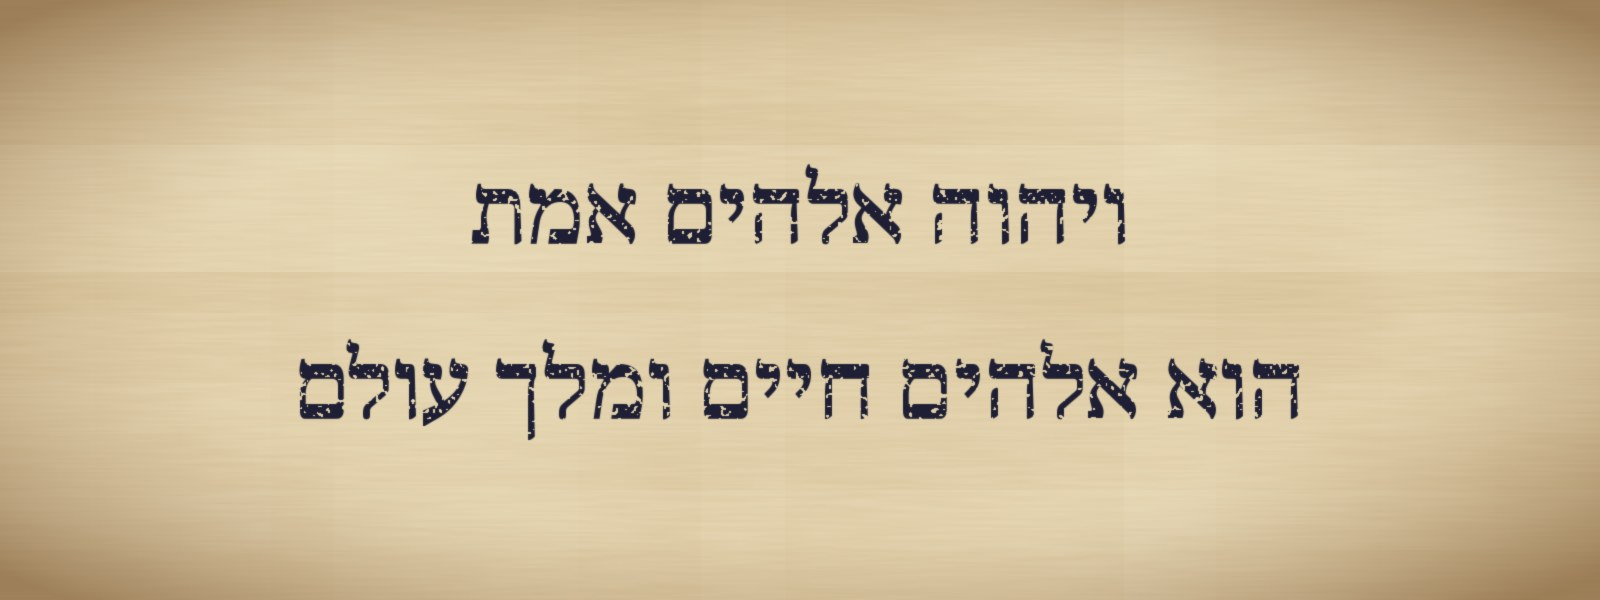
\includegraphics[width=0.80\linewidth,height=0.36\textheight,keepaspectratio]{portada.jpg}\\[-1pt]
  {\fontsize{5}{6}\selectfont\color{gris}\textit{Nota.} Elaboración propia: Jer 10:10 en texto hebreo consonántico (BHS).}}
\begin{document}
\frame{\titlepage}

\begin{frame}\frametitle{Contenidos}\tableofcontents\end{frame}

% ------------------------------------------------------------------
\section{Premisa}

\begin{frame}{``Toda verdad es verdad de Dios''}
\begin{columns}[c,onlytextwidth]
\begin{column}{0.50\textwidth}
\begin{tcolorbox}[colback=papiro,colframe=dorado,boxrule=1.2pt,arc=3pt]
\centering\small La verdad no es un constructo social ni una abstracción filosófica. Es la correspondencia exacta entre lo que creemos y \destacar{la realidad tal como Dios la concibió, la creó y la sostiene}.
\end{tcolorbox}
\small\RaggedRight Si Dios es la fuente de la verdad, todo lo verdadero del universo viene de él: la física, la política, la moral y la identidad del ser humano.
\end{column}
\begin{column}{0.48\textwidth}
\begin{cita}Le dijo Pilato: ¿Qué es la verdad?\fuente{(Jn 18:38, RVR1960)}\end{cita}
\scriptsize\grc{τί ἐστιν ἀλήθεια;} Pilato pregunta \emph{qué} es la verdad delante de \emph{quién} es la verdad (Jn 14:6). El estudio recorre ese camino: de la idea a la Persona.\par\smallskip
\precision{la frase ``toda verdad es verdad de Dios'' es la premisa de tu material; la tradición la remonta a Agustín, \emph{De doctrina christiana} II.18.28.}
\end{column}
\end{columns}
\end{frame}

\begin{frame}{El recorrido}
\centering
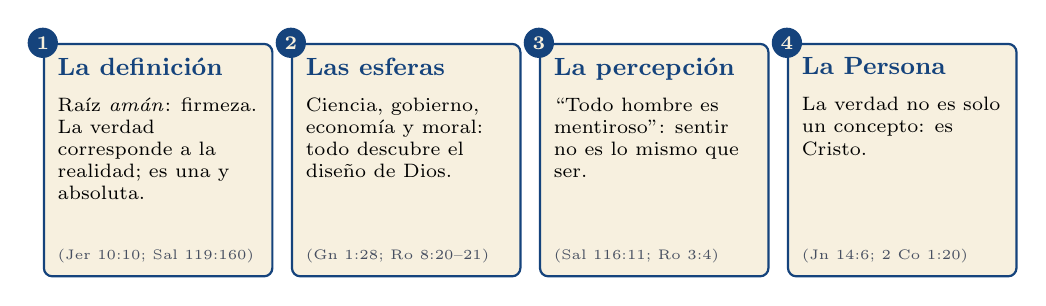
\begin{tikzpicture}
 \foreach \x/\n/\t/\d/\r in {0/1/{La definición}/{Raíz \emph{amán}: firmeza. La verdad corresponde a la realidad; es una y absoluta.}/{Jer 10:10; Sal 119:160},
   3.15/2/{Las esferas}/{Ciencia, gobierno, economía y moral: todo descubre el diseño de Dios.}/{Gn 1:28; Ro 8:20--21},
   6.3/3/{La percepción}/{``Todo hombre es mentiroso'': sentir no es lo mismo que ser.}/{Sal 116:11; Ro 3:4},
   9.45/4/{La Persona}/{La verdad no es solo un concepto: es Cristo.}/{Jn 14:6; 2 Co 1:20}}{
  \node[caja,anchor=north] (b\n) at (\x,0) {\parbox[t][2.6cm][t]{2.55cm}{\RaggedRight
    {\small\textbf{\textcolor{azul}{\t}}}\\[5pt]\scriptsize \d\par\vfill{\tiny\color{gris}(\r)}}};
  \node[circle,fill=azul,text=papiro,font=\scriptsize\bfseries,inner sep=1.6pt] at (b\n.north west) {\n};}
\end{tikzpicture}\par\medskip
\begin{cita}Mas alábese en esto el que se hubiere de alabar: en entenderme y conocerme, que yo soy \SENOR{}\ldots\fuente{(Jer 9:24 [9:23], RVR1960)}\end{cita}
\scriptsize Pocos versos después del verso clave de esta obra, Jeremías dice \emph{quién} es el Dios que se puede conocer: ``Mas \SENOR{} es el Dios verdadero'' (10:10).
\end{frame}

% ------------------------------------------------------------------
\section{Jeremías 10}

\begin{frame}{Ídolos que no hablan}
\begin{columns}[t,onlytextwidth]
\begin{column}{0.52\textwidth}
\begin{cita}Porque las costumbres de los pueblos son vanidad; porque leño del bosque cortaron, obra de manos de artífice con buril. Con plata y oro lo adornan; con clavos y martillo lo afirman para que no se mueva. Derechos están como palmera, y no hablan; son llevados, porque no pueden andar.\fuente{(Jer 10:3--5, RVR1960)}\end{cita}
\end{column}
\begin{column}{0.46\textwidth}\small
\begin{itemize}
\item Jeremías se burla: el ídolo necesita \destacar{clavos} para quedarse firme. Su ``firmeza'' es prestada.
\item No habla, no anda, no hace mal ni bien (10:5). Es ``vanidad'' (\heb{הֶבֶל}, \emph{hével}: vapor, soplo).
\item El capítulo opone dos ``firmezas'': la del ídolo clavado y la del Dios que es \emph{emet}.
\end{itemize}
\precision{el contraste ``firmeza clavada / firmeza de Dios'' es una lectura propia de esta serie.}
\end{column}
\end{columns}
\end{frame}

\begin{frame}{Texto ancla: Jer 10:10}
\fotolado{panel_jeremias10.jpg}{Elaboración propia: Jer 10:10a en texto hebreo consonántico (BHS).}
\begin{columns}[c,onlytextwidth]
\begin{column}{0.58\textwidth}
\begin{cita}No hay semejante a ti, oh \SENOR{}; grande eres tú, y grande tu nombre en poderío\ldots{} Mas \SENOR{} es el Dios verdadero; él es Dios vivo y Rey eterno; a su ira tiembla la tierra, y las naciones no pueden sufrir su indignación.\fuente{(Jer 10:6, 10, RVR1960)}\end{cita}
\begin{cita}Todo hombre se embrutece, y le falta ciencia; se avergüenza de su ídolo todo fundidor, porque mentirosa es su obra de fundición, y no hay espíritu en ella.\fuente{(Jer 10:14, RVR1960)}\end{cita}
\end{column}
\begin{column}{0.40\textwidth}\end{column}
\end{columns}
\end{frame}

\begin{frame}{Jer 10:10 en hebreo}
\begin{center}
\heb{וַיהוָה אֱלֹהִים אֱמֶת הוּא־אֱלֹהִים חַיִּים וּמֶלֶךְ עוֹלָם}\\[2pt]
\heb{מִקִּצְפּוֹ תִּרְעַשׁ הָאָרֶץ וְלֹא־יָכִלוּ גוֹיִם זַעְמוֹ}
\end{center}
\renewcommand{\arraystretch}{1.12}\scriptsize
\begin{tabular}{@{}>{\RaggedRight\arraybackslash}p{2.9cm}>{\RaggedRight\arraybackslash}p{1.2cm}>{\RaggedRight\arraybackslash}p{7.7cm}@{}}
\toprule
\textbf{Término} & \textbf{Raíz} & \textbf{Sentido} \\ \midrule
\heb{אֱלֹהִים אֱמֶת} \emph{Elohim emet} & \heb{אמן} & ``Dios verdad'': el sustantivo \emph{emet} califica a Dios. No dice que Dios \emph{tenga} verdad, sino que \emph{es} verdad. \\
\heb{אֱלֹהִים חַיִּים} \emph{Elohim jayyim} & \heb{חיה} & ``Dios vivo'': frente al ídolo en el que ``no hay espíritu'' (10:14). \\
\heb{מֶלֶךְ עוֹלָם} \emph{mélej olam} & \heb{מלך} & ``Rey eterno'': no lo ``llevan'' (10:5); él gobierna. \\
\heb{כִּי שֶׁקֶר נִסְכּוֹ} \emph{ki shéqer nisko} & \heb{שׁקר} & ``porque mentira es su (imagen) fundida'' (10:14): el ídolo es \emph{shéqer}. \\
\heb{הֶבֶל} \emph{hével} & \heb{הבל} & ``vanidad'', vapor (10:3, 8, 15). \\
\bottomrule
\end{tabular}\par\smallskip
\precision{la RVR1960 traduce ``el Dios verdadero''; el hebreo yuxtapone \emph{Elohim} y \emph{emet} (HALOT). Para los ídolos usa \emph{shéqer}, ``mentira, engaño''.}
\end{frame}

\begin{frame}{Jeremías 10: dos columnas que se alternan}
\centering
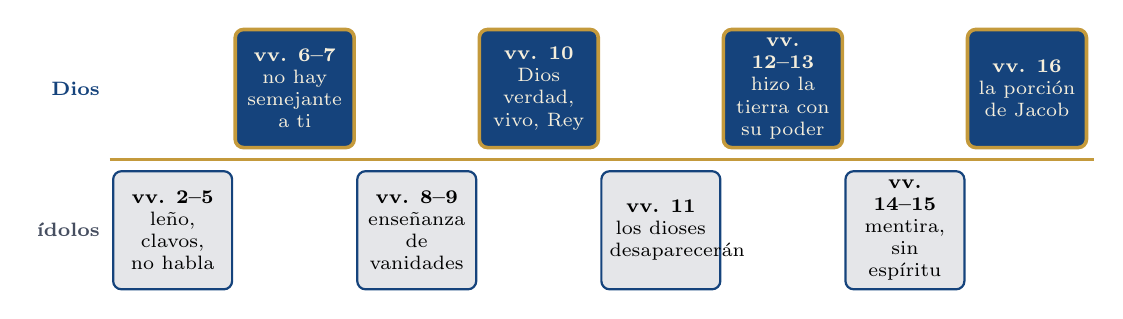
\begin{tikzpicture}[font=\scriptsize]
 \foreach \x/\v/\t in {1.55/{6--7}/{no hay semejante a ti}, 4.65/{10}/{Dios verdad, vivo, Rey}, 7.75/{12--13}/{hizo la tierra con su poder}, 10.85/{16}/{la porción de Jacob}}{
   \node[draw=dorado,line width=1.3pt,fill=azul,text=papiro,rounded corners=3pt,text width=1.3cm,align=center,inner sep=3pt,minimum height=1.5cm] at (\x,0.9) {\textbf{vv. \v}\\ \t};}
 \foreach \x/\v/\t in {0/{2--5}/{leño, clavos, no habla}, 3.1/{8--9}/{enseñanza de vanidades}, 6.2/{11}/{los dioses desaparecerán}, 9.3/{14--15}/{mentira, sin espíritu}}{
   \node[caja,fill=gris!15,text width=1.3cm,align=center,inner sep=3pt,minimum height=1.5cm] at (\x,-0.9) {\textbf{vv. \v}\\ \t};}
 \draw[dorado,line width=1pt] (-0.8,0) -- (11.7,0);
 \node[anchor=east,font=\scriptsize\bfseries,text=azul] at (-0.8,0.9) {Dios};
 \node[anchor=east,font=\scriptsize\bfseries,text=gris] at (-0.8,-0.9) {ídolos};
\end{tikzpicture}\par\medskip
\begin{columns}[t,onlytextwidth]
\begin{column}{0.49\textwidth}\small
El poema alterna como un juicio: cada descripción de los ídolos recibe una respuesta sobre el Dios verdadero. El centro (v. 10) es la confesión: \destacar{\emph{Elohim emet}}.
\end{column}
\begin{column}{0.49\textwidth}\scriptsize
El v. 11 está en \destacar{arameo}, la lengua internacional del imperio: es la frase que Israel debía decir a las naciones en su propio idioma: \heb{אֱלָהַיָּא דִּי־שְׁמַיָּא וְאַרְקָא לָא עֲבַדוּ}.\par\smallskip
\precision{la estructura alternada es una lectura de la composición del poema (Lundbom, 1999).}
\end{column}
\end{columns}
\end{frame}

\begin{frame}{Precisión textual: Jer 10 en la LXX y en Qumrán}
\scriptsize\renewcommand{\arraystretch}{1.2}
\begin{tabular}{@{}>{\RaggedRight\arraybackslash}p{3.1cm}>{\RaggedRight\arraybackslash}p{8.7cm}@{}}
\toprule
\textbf{Testigo} & \textbf{Jer 10:1--16} \\ \midrule
Texto masorético (BHS) & incluye los vv. 6--8 y 10 (las alabanzas al \SENOR). \\
Septuaginta & no tiene los vv. 6--8 ni el v. 10; pone el v. 9 después del 5a. Es la forma ``corta'' de Jeremías, alrededor de una séptima parte más breve que el TM. \\
4QJer\textsuperscript{b} (4Q71) & fragmento de Qumrán que coincide con la forma corta y el orden de la LXX. \\
4QJer\textsuperscript{a} (4Q70) & otro manuscrito de Qumrán que sigue la forma larga del TM. \\
\bottomrule
\end{tabular}\par\medskip
\small En Qumrán circulaban \destacar{las dos ediciones} de Jeremías. La RVR1960 sigue el texto masorético, que incluye el v. 10. La confesión del v. 10 está, además, en el resto de la Escritura: ``Dios vivo'' (Dt 5:26; Sal 42:2), ``Dios de verdad'' (Sal 31:5; Is 65:16).\par\smallskip
\precision{según Tov (2012), que usa Jer 10 como ejemplo clásico de dos ediciones literarias; las sigla y el contenido de los fragmentos se pueden cotejar en la Leon Levy Dead Sea Scrolls Digital Library.}
\end{frame}

% ------------------------------------------------------------------
\section{La palabra}

\begin{frame}{La raíz \heb{אמן} en lo concreto}
\begin{columns}[t,onlytextwidth]
\begin{column}{0.55\textwidth}
\scriptsize\renewcommand{\arraystretch}{1.16}
\begin{tabular}{@{}>{\RaggedRight\arraybackslash}p{2.0cm}>{\RaggedRight\arraybackslash}p{2.5cm}>{\RaggedRight\arraybackslash}p{1.6cm}@{}}
\toprule
\textbf{Forma} & \textbf{Uso concreto} & \textbf{Texto} \\ \midrule
\heb{הָאֹמֵן} \emph{ha'omén} & ``la que cría'': el que carga al niño & Nm 11:12 \\
\heb{אֹמֶנֶת} \emph{oménet} & ``aya'', nodriza & Rt 4:16 \\
\heb{אֹמְנוֹת} \emph{omnot} & ``quiciales'', soportes de las puertas & 2~R 18:16 \\
\heb{אֱמוּנָה} \emph{emuná} & ``firmeza'' de las manos de Moisés & Éx 17:12 \\
\heb{נֶאֱמָן} \emph{ne'emán} & ``lugar firme'' para un clavo & Is 22:23 \\
\heb{וְנֶאְמַן} \emph{vene'mán} & ``será afirmada'' tu casa & 2~S 7:16 \\
\bottomrule
\end{tabular}
\end{column}
\begin{column}{0.43\textwidth}
\begin{cita}\ldots{} y Aarón y Hur sostenían sus manos\ldots{} así hubo en sus manos firmeza hasta que se puso el sol.\fuente{(Éx 17:12, RVR1960)}\end{cita}
\small La raíz dice \destacar{sostener y ser sostenido}: el brazo que carga a un niño, el poste que sostiene una puerta, las manos que no caen.\par\smallskip
\precision{el sentido de una palabra lo fija su uso, no su etimología (Carson, 2013, ``falacia de la raíz''). Aquí el uso confirma la idea de firmeza que tu material le da a la raíz.}
\end{column}
\end{columns}
\end{frame}

\begin{frame}{Creer es apoyarse en lo firme}
\begin{columns}[c,onlytextwidth]
\begin{column}{0.50\textwidth}
\begin{cita}Si vosotros no creyereis, de cierto no permaneceréis.\fuente{(Is 7:9b, RVR1960)}\end{cita}
\begin{center}\heb{אִם לֹא תַאֲמִינוּ כִּי לֹא תֵאָמֵנוּ}\end{center}
\scriptsize\renewcommand{\arraystretch}{1.12}
\begin{tabular}{@{}>{\RaggedRight\arraybackslash}p{1.8cm}>{\RaggedRight\arraybackslash}p{4.0cm}@{}}
\toprule
\heb{תַאֲמִינוּ} & hifil: ``os apoyáis, creéis'' \\
\heb{תֵאָמֵנוּ} & nifal: ``seréis sostenidos, firmes'' \\
\bottomrule
\end{tabular}
\end{column}
\begin{column}{0.48\textwidth}\small
\begin{itemize}
\item Isaías juega con la misma raíz dos veces: ``si no os afirmáis, no seréis afirmados''.
\item \destacar{Creer} (\emph{he'emín}) es apoyar el peso en algo firme. \destacar{Verdad} (\emph{emet}) es lo que aguanta ese peso.
\item Por eso fe y verdad no se oponen: la fe se apoya en lo verdadero.
\end{itemize}
\precision{la LXX lee otra cosa: \grc{οὐδὲ μὴ συνῆτε}, ``tampoco entenderéis''. El juego de palabras solo existe en hebreo.}
\end{column}
\end{columns}
\end{frame}

\begin{frame}{Una raíz, una familia}
\centering
\begin{tikzpicture}[font=\scriptsize]
 \node[draw=dorado,line width=1.6pt,fill=azul,text=papiro,rounded corners=3pt,text width=2.6cm,align=center,inner sep=5pt] (r) at (0,0) {\heb{א־מ־ן}\\ \textbf{\emph{amán}}\\ sostener, ser firme};
 \foreach \a/\h/\t/\s/\x/\y in {a/{אֱמֶת}/{emet}/{verdad, firmeza (127)}/-4.6/1.3, b/{אֱמוּנָה}/{emuná}/{fidelidad, firmeza (49)}/-4.6/-1.3,
   c/{אָמֵן}/{amén}/{``así es'', ``firme'' (30)}/0/-2.25, d/{הֶאֱמִין}/{he'emín}/{creer, apoyarse}/4.6/1.3, e/{נֶאֱמָן}/{ne'emán}/{fiel, estable}/4.6/-1.3, f/{אָמְנָם}/{omnam}/{verdaderamente}/0/2.25}{
  \node[caja,text width=2.5cm,align=center] (\a) at (\x,\y) {\heb{\h}\ \textbf{\emph{\t}}\\ \s};
  \draw[dorado,line width=1pt] (r) -- (\a);}
\end{tikzpicture}\par\medskip
\small\RaggedRight Verdad, fidelidad, fe y amén son ramas del mismo tronco. Por eso la RVR1960 traduce \emph{emet} unas veces ``verdad'' y otras ``fidelidad'', y \emph{emuná} unas veces ``fidelidad'' y otras ``verdad''.\par\smallskip
\precision{conteos propios en la BHS con números Strong (\emph{emet} H571, \emph{emuná} H530, \emph{amén} H543); verificar en e-Sword.}
\end{frame}

\begin{frame}{El espectro completo: hebreo y arameo}
\scriptsize\renewcommand{\arraystretch}{1.13}
\begin{tabular}{@{}>{\RaggedRight\arraybackslash}p{2.9cm}>{\RaggedRight\arraybackslash}p{1.0cm}>{\RaggedRight\arraybackslash}p{4.4cm}>{\RaggedRight\arraybackslash}p{3.3cm}@{}}
\toprule
\textbf{Término} & \textbf{Veces} & \textbf{Cómo lo traduce la RVR1960} & \textbf{Textos} \\ \midrule
\heb{אֱמֶת} \emph{emet} & 127 & ``verdad'' ($\approx$\,93), ``verdadero/a'' (9), ``fidelidad'' (4), ``seguridad'', ``rectamente'' & Gn 24:27; Jer 10:10; Sal 31:5 \\
\heb{אֱמוּנָה} \emph{emuná} & 49 & ``fidelidad'' (13), ``verdad'' (18), ``firmeza'', ``fe'' & Éx 17:12; Dt 32:4; Hab 2:4 \\
\heb{אָמֵן} \emph{amén} & 30 & ``amén'' (28); ``Dios de verdad'' (2) & Dt 27:15; Is 65:16 \\
\heb{אֹמֶן} \emph{ómen} & 1 & ``firmeza'' & Is 25:1 \\
\heb{אָמְנָם}, \heb{אֻמְנָם} \emph{omnam} & 14 & ``verdaderamente'', ``de veras'' & 1~R 8:27; Job 19:4 \\
\heb{אָכֵן} \emph{ajén} & --- & ``verdaderamente'' & Is 45:15 \\
\heb{נָכוֹן} \emph{najón} & --- & ``cosa cierta'' (con \emph{emet}) & Dt 13:14; 17:4 \\
\heb{קֹשֶׁט} \emph{qóshet} & 2 & ``verdad'' & Pr 22:21 \\
arameo \heb{קְשֹׁט} \emph{qeshot} & 2 & ``verdaderas'', ``ciertamente'' & Dn 2:47; 4:37 \\
arameo \heb{יַצִּיב} \emph{yatsiv} & 5 & ``verdadero'', ``la verdad'' & Dn 2:45; 7:16 \\ \midrule
\heb{שֶׁקֶר} \emph{shéqer} & 113 & ``mentira, falsedad, engaño'' (lo contrario) & Jer 10:14; 28:15 \\
\heb{כָּזָב} \emph{kazav} & 31 & ``mentira''; el verbo: ``mentiroso'' & Sal 116:11; Is 28:17 \\
\bottomrule
\end{tabular}\par\smallskip
\precision{conteo propio (BHS y RVR1960 con Strong); las cifras de \emph{ajén} y \emph{najón} no se dan porque en la mayoría de sus usos no significan ``verdad''.}
\end{frame}

\begin{frame}{El espectro completo: griego y la RVR1960}
\begin{columns}[t,onlytextwidth]
\begin{column}{0.60\textwidth}
\scriptsize\renewcommand{\arraystretch}{1.13}
\begin{tabular}{@{}>{\RaggedRight\arraybackslash}p{1.8cm}>{\RaggedRight\arraybackslash}p{0.7cm}>{\RaggedRight\arraybackslash}p{2.3cm}>{\RaggedRight\arraybackslash}p{2.0cm}@{}}
\toprule
\textbf{Término} & \textbf{NA27} & \textbf{Sentido} & \textbf{Textos} \\ \midrule
\grc{ἀλήθεια} & 109 & verdad & Jn 14:6; Ro 1:25 \\
\grc{ἀληθής} & 26 & veraz, verdadero & Ro 3:4; Jn 8:26 \\
\grc{ἀληθινός} & 28 & genuino, real & 1 Ts 1:9; Jn 15:1 \\
\grc{ἀληθῶς} & 18 & verdaderamente & 1 Ts 2:13 \\
\grc{ἀληθεύω} & 2 & decir (seguir) la verdad & Gá 4:16; Ef 4:15 \\
\grc{ἀψευδής} & 1 & que no miente & Tit 1:2 \\
\grc{ἀμήν} & 128 & amén; ``de cierto'' & 2 Co 1:20; Ap 3:14 \\ \midrule
\grc{ψεῦδος}, \grc{ψεύστης} & 10; 10 & mentira; mentiroso & Ro 1:25; Jn 8:44 \\
\bottomrule
\end{tabular}
\end{column}
\begin{column}{0.38\textwidth}\small
\textbf{En la RVR1960:} ``verdad'' y sus formas aparecen \destacar{432 veces en 406 versículos}: 188 en el AT y 244 en el NT.\par\smallskip
\scriptsize\renewcommand{\arraystretch}{1.1}
\begin{tabular}{@{}lr@{}}
verdad / verdades & 335 \\
verdadero/a/os/as & 65 \\
verdaderamente & 27 \\
veraz / veraces & 5 \\
\end{tabular}\par\smallskip
\precision{57 veces aparece ``a la verdad'', un giro que casi siempre traduce la partícula griega \grc{μέν} (``por cierto'') y no habla de la verdad. Conteo propio, sin títulos de sección.}
\end{column}
\end{columns}
\end{frame}

\begin{frame}{Una palabra, dos traducciones}
\scriptsize\renewcommand{\arraystretch}{1.2}
\begin{tabular}{@{}>{\RaggedRight\arraybackslash}p{1.5cm}>{\RaggedRight\arraybackslash}p{1.7cm}>{\RaggedRight\arraybackslash}p{2.9cm}>{\RaggedRight\arraybackslash}p{2.6cm}>{\RaggedRight\arraybackslash}p{2.8cm}@{}}
\toprule
\textbf{Texto} & \textbf{Original} & \textbf{RVR1960} & \textbf{LBLA} & \textbf{NVI} \\ \midrule
Sal 119:30 & \heb{דֶּרֶךְ־אֱמוּנָה} & ``el camino de la verdad'' & ``el camino de la verdad'' & ``el camino de la fidelidad'' \\
Sal 119:160 & \heb{רֹאשׁ־דְּבָרְךָ אֱמֶת} & ``La suma de tu palabra es verdad'' & ``La suma de tu palabra es verdad'' & ``La suma de tus palabras es la verdad'' \\
Jer 5:1 & \heb{מְבַקֵּשׁ אֱמוּנָה} & ``que busque verdad'' & ``que busque la verdad'' & ``y busque la verdad'' \\
3~Jn 3 & \grc{τῇ ἀληθείᾳ} & ``tu verdad'' & ``tu verdad'' & ``tu fidelidad'' \\
\bottomrule
\end{tabular}\par\medskip
\begin{columns}[t,onlytextwidth]
\begin{column}{0.49\textwidth}\small
Las versiones no se contradicen: eligen uno de los dos lados de la misma raíz. En hebreo, ser verdadero es \destacar{ser confiable}.
\end{column}
\begin{column}{0.49\textwidth}\scriptsize
\heb{רֹאשׁ} (\emph{rosh}) es ``cabeza'': la ``suma'' (el total, como al contar cabezas) o el ``principio''. La RV1909 y tu material leen ``El principio de tu palabra es verdad''.\par\smallskip
\precision{la NVI y la LBLA se citan desde tu compendio; la RV1909 desde la biblioteca de la serie.}
\end{column}
\end{columns}
\end{frame}

\begin{frame}{La primera vez: el siervo de Abraham}
\begin{columns}[t,onlytextwidth]
\begin{column}{0.52\textwidth}
\begin{cita}y dijo: Bendito sea \SENOR{}, Dios de mi amo Abraham, que no apartó de mi amo su misericordia y su verdad, guiándome \SENOR{} en el camino a casa de los hermanos de mi amo.\fuente{(Gn 24:27, RVR1960)}\end{cita}
\begin{center}\heb{אֲשֶׁר לֹא־עָזַב חַסְדּוֹ וַאֲמִתּוֹ}\end{center}
\end{column}
\begin{column}{0.46\textwidth}\small
\begin{itemize}
\item Es la primera aparición de \emph{emet} en la Biblia, y llega en pareja: \emph{jésed ve'emet}, ``amor leal y verdad'' (cf. Éx 34:6).
\item El siervo había orado por una señal (24:12--14); Dios respondió \destacar{tal como dijo}.
\item Después repite: ``me había guiado por \destacar{camino de verdad}'' (\heb{בְּדֶרֶךְ אֱמֶת}, 24:48): el camino correcto, el que llega.
\end{itemize}
\precision{conteo propio con Strong H571: Gn 24:27 es la primera aparición en el orden canónico.}
\end{column}
\end{columns}
\end{frame}

\begin{frame}{El Dios del Amén}
\fotolado{panel_isaias65.jpg}{Elaboración propia: Is 65:16 en texto hebreo consonántico (BHS).}
\begin{columns}[c,onlytextwidth]
\begin{column}{0.58\textwidth}
\begin{cita}El que se bendijere en la tierra, en el Dios de verdad se bendecirá; y el que jurare en la tierra, por el Dios de verdad jurará; porque las angustias primeras serán olvidadas.\fuente{(Is 65:16, RVR1960)}\end{cita}
\begin{center}\heb{יִתְבָּרֵךְ בֵּאלֹהֵי אָמֵן}\end{center}
\scriptsize\renewcommand{\arraystretch}{1.12}
\begin{tabular}{@{}>{\RaggedRight\arraybackslash}p{2.0cm}>{\RaggedRight\arraybackslash}p{4.7cm}@{}}
\toprule
\heb{אֱלֹהֵי אָמֵן} & literalmente ``el Dios del Amén'' \\
LXX & \grc{τὸν θεὸν τὸν ἀληθινόν}, ``el Dios verdadero'' \\
contexto & cielos nuevos y tierra nueva (65:17) \\
\bottomrule
\end{tabular}\par\smallskip
El Dios que dice ``amén'' a su propia palabra: lo que promete, es.
\end{column}
\begin{column}{0.40\textwidth}\end{column}
\end{columns}
\end{frame}



\begin{frame}{Lo que permanece y lo que dura un momento}
\begin{columns}[c,onlytextwidth]
\begin{column}{0.50\textwidth}
\begin{cita}El labio veraz permanecerá para siempre; Mas la lengua mentirosa sólo por un momento.\fuente{(Pr 12:19, RVR1960)}\end{cita}
\begin{center}\heb{שְׂפַת־אֱמֶת תִּכּוֹן לָעַד}\\ \heb{וְעַד־אַרְגִּיעָה לְשׁוֹן שָׁקֶר}\end{center}
\end{column}
\begin{column}{0.48\textwidth}
\scriptsize\renewcommand{\arraystretch}{1.15}
\begin{tabular}{@{}>{\RaggedRight\arraybackslash}p{1.9cm}>{\RaggedRight\arraybackslash}p{3.3cm}@{}}
\toprule
\heb{תִּכּוֹן} \emph{tikkón} & ``estará firme'' (\heb{כון}, establecer) \\
\heb{לָעַד} \emph{la'ad} & ``para siempre'' \\
\heb{אַרְגִּיעָה} \emph{argi'á} & ``un parpadeo'', un instante \\
\bottomrule
\end{tabular}\par\medskip
\small El proverbio mide la verdad por su \destacar{duración}: la verdad queda en pie; la mentira dura un parpadeo. Es la ``plomada'' en el tiempo.
\end{column}
\end{columns}
\end{frame}

\begin{frame}{Del hebreo a Pablo}
\centering
\begin{tikzpicture}[font=\scriptsize,node distance=0.7cm]
 \node[caja,text width=3.1cm,align=center] (h) {\textbf{Hebreo}\\ \heb{אֱמֶת} \emph{emet}\\ \heb{אָמֵן} \emph{amén}\\ \heb{אֱמוּנָה} \emph{emuná}};
 \node[caja,text width=3.1cm,align=center,right=of h] (l) {\textbf{Septuaginta}\\ \grc{ἀλήθεια} (casi siempre)\\ \grc{ἀληθινός} (Is 65:16)\\ \grc{πίστις}, \grc{ἀλήθεια}};
 \node[caja,text width=3.1cm,align=center,right=of l] (p) {\textbf{Pablo}\\ \grc{ὁ θεὸς ἀληθής} (Ro 3:4)\\ \grc{θεῷ ζῶντι καὶ ἀληθινῷ} (1 Ts 1:9)\\ \grc{τὸ ἀμήν} (2 Co 1:20)};
 \draw[-{Latex[length=2.5mm]},dorado,line width=1.2pt] (h)--(l);
 \draw[-{Latex[length=2.5mm]},dorado,line width=1.2pt] (l)--(p);
\end{tikzpicture}\par\medskip
\scriptsize\renewcommand{\arraystretch}{1.15}
\begin{tabular}{@{}>{\RaggedRight\arraybackslash}p{2.6cm}>{\RaggedRight\arraybackslash}p{9.2cm}@{}}
\toprule
\grc{ἀλήθεια} \emph{alétheia} & en griego clásico, lo real frente a la apariencia; en la LXX y en Pablo carga además el sentido hebreo de \emph{firmeza y fidelidad} (Ro 3:3--4; 15:8). \\
\grc{ἀληθινός} \emph{alēthinós} & ``genuino, real'': el Dios verdadero frente a los ídolos (1 Ts 1:9; Jn 17:3). \\
\grc{ἀμήν} \emph{amén} & transliteración del hebreo: Pablo lo deja sin traducir. \\
\bottomrule
\end{tabular}\par\smallskip
\precision{se suele explicar \grc{ἀλήθεια} como \emph{a-lēthē}, ``lo no oculto''; esa etimología es discutida y no decide su sentido bíblico (Carson, 2013).}
\end{frame}

% ------------------------------------------------------------------
\section{Definición}

\begin{frame}{``Lo que corresponde a la realidad''}
\begin{columns}[c,onlytextwidth]
\begin{column}{0.50\textwidth}
\begin{tcolorbox}[colback=papiro,colframe=dorado,boxrule=1.2pt,arc=3pt]
\centering\small ``La verdad es lo que corresponde a la realidad.''
\end{tcolorbox}
\small\RaggedRight Si una idea, un sentimiento o una estructura no corresponde a la realidad \destacar{tal como Dios la ve, la concibió y la diseñó}, carece de firmeza y no es verdad.
\end{column}
\begin{column}{0.48\textwidth}
\centering
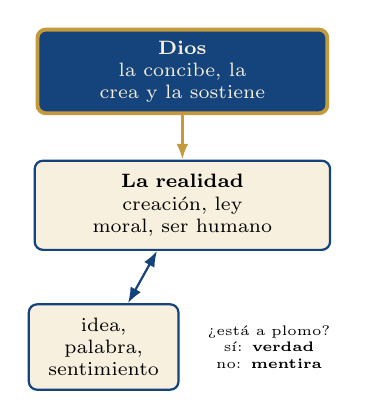
\begin{tikzpicture}[font=\scriptsize]
 \node[draw=dorado,line width=1.4pt,fill=azul,text=papiro,rounded corners=3pt,text width=3.4cm,align=center,inner sep=4pt] (d) at (0,2.0) {\textbf{Dios}\\ la concibe, la crea y la sostiene};
 \node[caja,text width=3.4cm,align=center] (r) at (0,0.3) {\textbf{La realidad}\\ creación, ley moral, ser humano};
 \node[caja,text width=1.55cm,align=center] (i) at (-1.0,-1.5) {idea, palabra, sentimiento};
 \node[text width=1.6cm,align=center,font=\tiny] at (1.1,-1.5) {¿está a plomo?\\ sí: \textbf{verdad}\\ no: \textbf{mentira}};
 \draw[-{Latex[length=2mm]},dorado,line width=1pt](d)--(r);
 \draw[{Latex[length=2mm]}-{Latex[length=2mm]},azul,line width=0.8pt](i)--(r);
\end{tikzpicture}
\end{column}
\end{columns}\par\medskip
\precision{la definición de la verdad como correspondencia es la clásica en filosofía; tu material le agrega lo decisivo: la medida es la realidad \emph{según Dios}, no según el observador.}
\end{frame}

\begin{frame}{Qué es la verdad de Dios}
\begin{tcolorbox}[colback=papiro,colframe=azul,boxrule=1pt,arc=3pt,fonttitle=\bfseries\small,title=Definición]
\small La verdad de Dios es la perfección eterna por la cual Dios \destacar{es real y firme}, \destacar{dice lo que es} y \destacar{cumple lo que dice}. Su palabra corresponde exactamente a la realidad que él mismo creó y sostiene; por eso él es la medida de toda verdad (Jer 10:10; Nm 23:19; Jn 14:6).
\end{tcolorbox}
\scriptsize\renewcommand{\arraystretch}{1.18}
\begin{tabular}{@{}>{\RaggedRight\arraybackslash}p{2.4cm}>{\RaggedRight\arraybackslash}p{5.6cm}>{\RaggedRight\arraybackslash}p{3.6cm}@{}}
\toprule
\textbf{Rasgo} & \textbf{Qué afirma} & \textbf{Textos} \\ \midrule
Real & es el Dios vivo, no una imagen & Jer 10:10; 1 Ts 1:9 \\
Firme (\emph{emet}) & lo que dice se sostiene & Sal 119:160; Pr 12:19 \\
Veraz & no miente ni puede mentir & Nm 23:19; Tit 1:2; He 6:18 \\
Fiel (\emph{emuná}) & cumple sus promesas & Mi 7:20; Ro 15:8 \\
Una & no dice ``sí'' y ``no'' a la vez & 2 Co 1:18--19 \\
Encarnada & la verdad tiene rostro & Jn 1:14; 14:6 \\
\bottomrule
\end{tabular}\par\smallskip
\begin{center}\footnotesize
\begin{tabular}{ll}
\textbf{Clasificación:} & Relación con el ser humano (¿cómo se revela?)\\
\textbf{Tipo:} & \destacar{incomunicable} como fuente; \destacar{comunicable} como veracidad (Ef 4:25)\\
\end{tabular}
\end{center}
\end{frame}

\begin{frame}{La verdad es una}
\begin{columns}[c,onlytextwidth]
\begin{column}{0.48\textwidth}
\centering
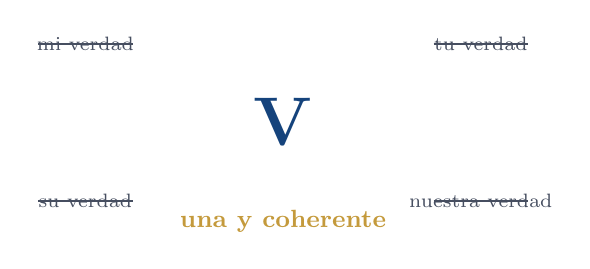
\begin{tikzpicture}
 \node[font=\fontsize{60}{60}\selectfont\bfseries,text=azul] (v) at (0,0) {V};
 \node[font=\small\bfseries,text=dorado] at (0,-1.25) {una y coherente};
 \foreach \a/\t in {150/{mi verdad},30/{tu verdad},210/{su verdad},330/{nuestra verdad}}{
  \node[font=\scriptsize,text=gris] (n\a) at (\a:2.9cm and 2.0cm) {\t};
  \draw[gris,line width=0.8pt] ($(n\a.south west)!0.5!(n\a.north east)+(-0.6,0)$) -- ++(1.2,0);}
\end{tikzpicture}
\end{column}
\begin{column}{0.50\textwidth}\small
\begin{itemize}
\item La verdad es \destacar{singular}, no plural: se escribe con ``V'' mayúscula y se mantiene unida.
\item El cristianismo no ofrece ``múltiples verdades'': presenta una visión del mundo coherente consigo misma.
\item Dios no es ``Sí y No'' (2 Co 1:18--19): su palabra no se contradice.
\end{itemize}
\begin{cita}Santifícalos en tu verdad; tu palabra es verdad.\fuente{(Jn 17:17, RVR1960)}\end{cita}
\end{column}
\end{columns}
\end{frame}

\begin{frame}{Dios es luz}
\begin{columns}[t,onlytextwidth]
\begin{column}{0.54\textwidth}
\begin{cita}Este es el mensaje que hemos oído de él, y os anunciamos: Dios es luz, y no hay ningunas tinieblas en él. Si decimos que tenemos comunión con él, y andamos en tinieblas, mentimos, y no practicamos la verdad.\fuente{(1~Jn 1:5--6, RVR1960)}\end{cita}
\scriptsize\grc{ὁ θεὸς φῶς ἐστιν}: Dios no tiene luz, \emph{es} luz. \grc{σκοτία ἐν αὐτῷ οὐκ ἔστιν οὐδεμία}: doble negación, ``no hay tiniebla, ninguna''. \grc{οὐ ποιοῦμεν τὴν ἀλήθειαν}: ``no hacemos la verdad''.
\end{column}
\begin{column}{0.44\textwidth}
\centering
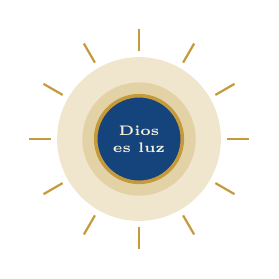
\begin{tikzpicture}[font=\scriptsize,scale=0.8]
 \fill[dorado!25] (0,0) circle (1.3);
 \fill[dorado!45] (0,0) circle (0.9);
 \node[draw=dorado,line width=1.3pt,fill=azul,text=papiro,circle,minimum size=1.1cm,align=center,font=\tiny\bfseries] at (0,0) {Dios\\ es luz};
 \foreach \a in {0,30,...,330}{\draw[dorado,line width=0.8pt] (\a:1.4) -- (\a:1.75);}
\end{tikzpicture}\par\smallskip
\small Sin una sola sombra: lo que Dios es, dice y hace coincide por completo. Por eso, en Juan, decir una cosa y andar en otra es \destacar{mentir}: la verdad también se \emph{hace} (Jn 3:21).
\end{column}
\end{columns}
\end{frame}

\begin{frame}{Sin sombra de variación, sin doblez}
\begin{columns}[t,onlytextwidth]
\begin{column}{0.49\textwidth}
\begin{cita}Toda buena dádiva y todo don perfecto desciende de lo alto, del Padre de las luces, en el cual no hay mudanza, ni sombra de variación.\fuente{(Stg 1:17, RVR1960)}\end{cita}
\scriptsize\grc{οὐκ ἔνι παραλλαγὴ ἢ τροπῆς ἀποσκίασμα}: el sol proyecta sombras que cambian con su giro; el Padre de las luces, no. Su verdad no varía con la hora ni con el ángulo.
\end{column}
\begin{column}{0.49\textwidth}
\begin{cita}Habla mentira cada uno con su prójimo; Hablan con labios lisonjeros, y con doblez de corazón.\fuente{(Sal 12:2 [12:3], RVR1960)}\end{cita}
\scriptsize\heb{בְּלֵב וָלֵב} (\emph{belev valev}): ``con un corazón y un corazón''. La doblez es tener dos corazones; Santiago lo llama \grc{δίψυχος}, ``de doble alma'' (Stg 1:8).
\end{column}
\end{columns}
\end{frame}

\begin{frame}{Luz: una verdad absoluta y sin doblez}
\begin{columns}[t,onlytextwidth]
\begin{column}{0.52\textwidth}\small
\begin{itemize}
\item Porque Dios es luz, su verdad es \destacar{absoluta}: no hay en él una zona oscura donde lo dicho deje de valer.
\item Porque no tiene sombra de variación, su verdad es \destacar{sin doblez}: no dice ``Sí y No'' (2 Co 1:17--18).
\item Y el que anda en su luz no puede tener dos corazones: ``Sea vuestro hablar: Sí, sí; no, no'' (Mt 5:37).
\end{itemize}
\end{column}
\begin{column}{0.46\textwidth}
\begin{cita}ahora sois luz en el Señor; andad como hijos de luz (porque el fruto del Espíritu es en toda bondad, justicia y verdad).\fuente{(Ef 5:8--9, RVR1960)}\end{cita}
\begin{cita}Envía tu luz y tu verdad; éstas me guiarán.\fuente{(Sal 43:3, RVR1960)}\end{cita}
\end{column}
\end{columns}\par\smallskip
\precision{en Ef 5:9 NA28 lee \grc{ὁ καρπὸς τοῦ φωτός}, ``el fruto de la luz''; la RVR1960 sigue el Texto Recibido, ``del Espíritu''.}
\end{frame}


\begin{frame}{Antídoto al relativismo}
\begin{columns}[t,onlytextwidth]
\begin{column}{0.49\textwidth}
\begin{tcolorbox}[colback=gris!12,colframe=gris,boxrule=0.8pt,arc=3pt,fonttitle=\bfseries\small,title=Rechazo]
\small La verdad \textbf{no} es relativa a la cultura, al individuo ni a lo pragmático (``lo que funciona'').
\end{tcolorbox}
\begin{tcolorbox}[colback=papiro,colframe=azul,boxrule=1pt,arc=3pt,fonttitle=\bfseries\small,title=Afirmación]
\small La verdad de Dios es absoluta y eterna, ``tan absoluta como la muerte o como la gravedad''. No cambia con la opinión de la sociedad: lo que Dios llamó profano en el siglo I lo sigue siendo hoy.
\end{tcolorbox}
\end{column}
\begin{column}{0.49\textwidth}
\begin{cita}Para siempre, oh \SENOR{}, Permanece tu palabra en los cielos.\fuente{(Sal 119:89, RVR1960)}\end{cita}
\begin{cita}La suma de tu palabra es verdad, Y eterno es todo juicio de tu justicia.\fuente{(Sal 119:160, RVR1960)}\end{cita}
\scriptsize Núñez (2020, cap. 1) recoge la expresión de Francis Schaeffer, ``la verdadera verdad'', contra la idea de que cada uno tiene su propia verdad: la verdad ``no es nuestra, sino que es únicamente de Dios''.
\end{column}
\end{columns}
\end{frame}

% ------------------------------------------------------------------
\section{La plomada}

\begin{frame}{La plomada: cómo funciona}
\begin{columns}[c,onlytextwidth]
\begin{column}{0.50\textwidth}
\centering
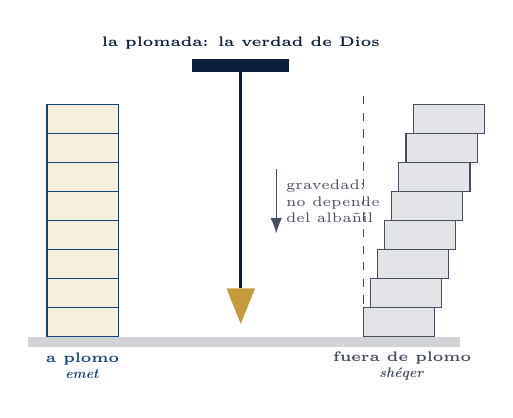
\begin{tikzpicture}[scale=0.82]
 % suelo
 \fill[gris!25] (-3.3,-0.15) rectangle (3.4,0);
 % muro a plomo (izquierda)
 \foreach \y in {0,0.45,...,3.2}{\draw[azul,fill=papiro] (-3.0,\y) rectangle (-1.9,\y+0.45);}
 \node[font=\tiny\bfseries,text=azul,align=center] at (-2.45,-0.45) {a plomo\\ \emph{emet}};
 % plomada (centro)
 \fill[azuloscuro] (-0.75,4.1) rectangle (0.75,4.3);
 \draw[azuloscuro,line width=1pt] (0,4.1) -- (0,0.75);
 \fill[dorado] (-0.22,0.75) -- (0.22,0.75) -- (0,0.2) -- cycle;
 \node[font=\tiny\bfseries,text=azuloscuro,align=center] at (0,4.55) {la plomada: la verdad de Dios};
 \draw[-{Latex[length=2mm]},gris] (0.55,2.6) -- (0.55,1.6) node[midway,right,font=\tiny,text=gris,align=left] {gravedad:\\ no depende\\ del albañil};
 % muro torcido (derecha)
 \foreach \i in {0,...,7}{\pgfmathsetmacro{\dx}{0.11*\i}\draw[gris,fill=gris!15] (1.9+\dx,0.45*\i) rectangle (3.0+\dx,0.45*\i+0.45);}
 \node[font=\tiny\bfseries,text=gris,align=center] at (2.5,-0.45) {fuera de plomo\\ \emph{shéqer}};
 \draw[gris,dashed] (1.9,0) -- (1.9,3.8);
\end{tikzpicture}
\end{column}
\begin{column}{0.48\textwidth}\small
\begin{itemize}
\item La plomada es un peso que cuelga de un cordel. La gravedad la pone siempre en la \destacar{vertical exacta}: no depende de la opinión del albañil.
\item \destacar{No se ajusta al muro}; el muro se ajusta a ella. El albañil que la ignora construye un muro que tarde o temprano cae.
\item Así es la verdad de Dios: mide la verticalidad de lo que existe, de lo que creemos y de lo que hacemos. Lo que no está a plomo es mentira y está destinado al colapso.
\end{itemize}
\precision{la imagen es de tu material; la Escritura la usa en Am 7:7--8, Is 28:17 y 2~R 21:13.}
\end{column}
\end{columns}
\end{frame}

\begin{frame}{La verticalidad de la verdad}
\centering
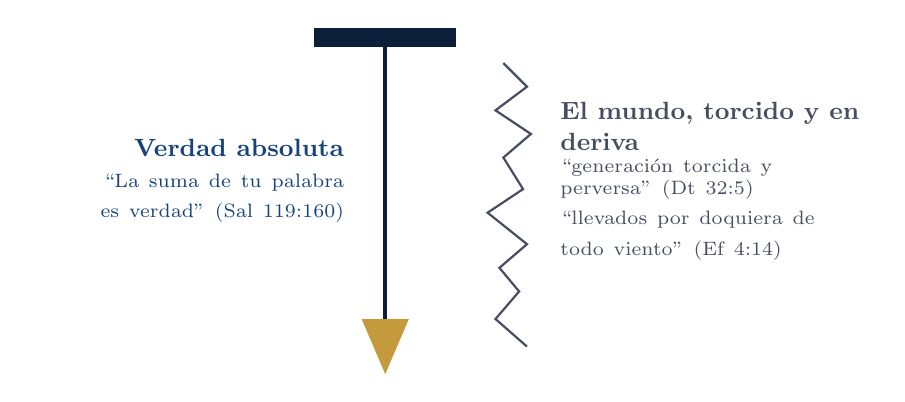
\begin{tikzpicture}[font=\scriptsize,xshift=-1cm]
 \fill[azuloscuro] (-0.9,4.0) rectangle (0.9,4.25);
 \draw[azuloscuro,line width=1.4pt] (0,4.0) -- (0,0.55);
 \fill[dorado] (-0.3,0.55) -- (0.3,0.55) -- (0,-0.15) -- cycle;
 \node[anchor=east,align=right,text=azul,font=\small\bfseries,text width=3.9cm] at (-0.4,2.3) {Verdad absoluta\\ \normalfont\scriptsize ``La suma de tu palabra es verdad'' (Sal 119:160)};
 \draw[gris,line width=0.8pt] (1.5,3.8) -- (1.8,3.5) -- (1.4,3.2) -- (1.85,2.9) -- (1.5,2.6) -- (1.75,2.2) -- (1.3,1.9) -- (1.8,1.5) -- (1.45,1.2) -- (1.7,0.9) -- (1.4,0.55) -- (1.8,0.2);
 \node[anchor=west,align=left,text=gris,font=\small\bfseries,text width=3.9cm] at (2.1,2.3) {El mundo, torcido y en deriva\\ \normalfont\scriptsize ``generación torcida y perversa'' (Dt 32:5)\\ \scriptsize ``llevados por doquiera de todo viento'' (Ef 4:14)};
\end{tikzpicture}\par\medskip
\begin{columns}[t,onlytextwidth]
\begin{column}{0.49\textwidth}
\begin{cita}Todos se desviaron, a una se han corrompido; No hay quien haga lo bueno, no hay ni siquiera uno.\fuente{(Sal 14:3, RVR1960)}\end{cita}
\end{column}
\begin{column}{0.49\textwidth}\scriptsize
\heb{הַכֹּל סָר}: ``todos se apartaron'' (\emph{sar}, salirse del camino). Pablo lo cita en Ro 3:12: \grc{πάντες ἐξέκλιναν}, ``todos se \emph{inclinaron} fuera'': nadie quedó a plomo.\par\smallskip
\precision{tu material cita el salmo con otra versión (``se han vuelto inútiles'' es la forma de Ro 3:12); aquí va la RVR1960.}
\end{column}
\end{columns}
\end{frame}

\begin{frame}{Recto y torcido}
\begin{columns}[t,onlytextwidth]
\begin{column}{0.50\textwidth}
\begin{cita}El es la Roca, cuya obra es perfecta, Porque todos sus caminos son rectitud; Dios de verdad, y sin ninguna iniquidad en él; Es justo y recto. La corrupción no es suya; de sus hijos es la mancha, Generación torcida y perversa.\fuente{(Dt 32:4--5, RVR1960)}\end{cita}
\begin{cita}Dios hizo al hombre recto, pero ellos buscaron muchas perversiones.\fuente{(Ec 7:29, RVR1960)}\end{cita}
\end{column}
\begin{column}{0.48\textwidth}
\scriptsize\renewcommand{\arraystretch}{1.13}
\begin{tabular}{@{}>{\RaggedRight\arraybackslash}p{2.1cm}>{\RaggedRight\arraybackslash}p{3.3cm}@{}}
\toprule
\heb{אֵל אֱמוּנָה} \emph{El emuná} & ``Dios de verdad'', de firmeza \\
\heb{יָשָׁר} \emph{yashar} & ``recto'': derecho, a plomo \\
\heb{דּוֹר עִקֵּשׁ וּפְתַלְתֹּל} & ``generación torcida y retorcida'' \\
LXX & \grc{γενεὰ σκολιὰ καὶ διεστραμμένη} \\
\bottomrule
\end{tabular}\par\medskip
\small Moisés canta la plomada: Dios es \emph{yashar}, la vertical; el pueblo es \emph{iqqesh}, lo torcido.\par\smallskip
\scriptsize Pablo toma estas palabras para la iglesia: ``hijos de Dios sin mancha en medio de una generación \grc{σκολιᾶς καὶ διεστραμμένης}\ldots{} resplandecéis como luminares'' (Flp 2:15).
\end{column}
\end{columns}
\end{frame}

\begin{frame}{La plomada en la Escritura}
\begin{columns}[t,onlytextwidth]
\begin{column}{0.50\textwidth}
\begin{cita}He aquí el Señor estaba sobre un muro hecho a plomo, y en su mano una plomada de albañil\ldots{} He aquí, yo pongo plomada de albañil en medio de mi pueblo Israel.\fuente{(Am 7:7--8, RVR1960)}\end{cita}
\begin{cita}He aquí que yo he puesto en Sion por fundamento una piedra, piedra probada, angular, preciosa, de cimiento estable; el que creyere, no se apresure. Y ajustaré el juicio a cordel, y a nivel la justicia; y granizo barrerá el refugio de la mentira.\fuente{(Is 28:16--17, RVR1960)}\end{cita}
\end{column}
\begin{column}{0.48\textwidth}
\scriptsize\renewcommand{\arraystretch}{1.12}
\begin{tabular}{@{}>{\RaggedRight\arraybackslash}p{1.9cm}>{\RaggedRight\arraybackslash}p{3.5cm}@{}}
\toprule
\heb{אֲנָךְ} \emph{anaj} & ``plomada'' (Am 7:7--8, sus 4 usos) \\
\heb{מִשְׁקֶלֶת} \emph{mishquélet} & ``nivel, plomada'' (Is 28:17; 2~R 21:13) \\
\heb{קַו} \emph{qav} & ``cordel'' de medir \\
\heb{הַמַּאֲמִין} \emph{hama'amín} & ``el que creyere'': raíz \emph{amán} \\
\heb{מַחְסֵה כָזָב} & ``refugio de la mentira'' \\
\bottomrule
\end{tabular}\par\medskip
\small Tu imagen de la verdad como \destacar{plomada} está en los profetas: Dios mide a su pueblo con su propia rectitud, y lo que no está a plomo cae.\par\smallskip
\precision{el sentido de \emph{anaj} se discute: HALOT propone ``estaño'' (acadio \emph{anāku}). \emph{Mishquélet} sí es plomada o nivel.}
\end{column}
\end{columns}
\end{frame}

\begin{frame}{El muro que se cae de repente}
\begin{columns}[c,onlytextwidth]
\begin{column}{0.52\textwidth}
\begin{cita}Porque desechasteis esta palabra, y confiasteis en violencia y en iniquidad, y en ello os habéis apoyado; por tanto, os será este pecado como grieta que amenaza ruina, extendiéndose en una pared elevada, cuya caída viene súbita y repentinamente.\fuente{(Is 30:12--13, RVR1960)}\end{cita}
\scriptsize\heb{כְּפֶרֶץ נֹפֵל נִבְעֶה בְּחוֹמָה נִשְׂגָּבָה}: ``como brecha que cae, abombada en un muro alto''. El pecado es un muro fuera de plomo: se ve firme hasta el día en que cae.
\end{column}
\begin{column}{0.46\textwidth}
\centering
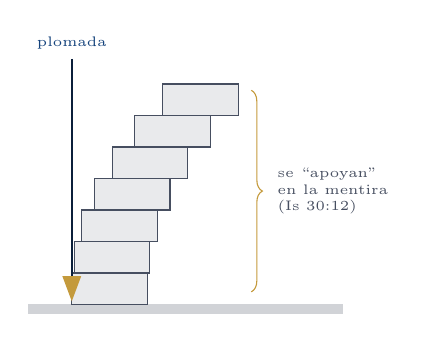
\begin{tikzpicture}[scale=0.8]
 \fill[gris!25] (-0.4,-0.15) rectangle (4.6,0);
 \foreach \i in {0,...,6}{\pgfmathsetmacro{\dx}{0.04*\i*\i}\draw[gris,fill=gris!12] (0.3+\dx,0.5*\i) rectangle (1.5+\dx,0.5*\i+0.5);}
 \draw[azuloscuro,line width=0.9pt] (0.3,3.9) -- (0.3,0.45);
 \fill[dorado] (0.15,0.45) -- (0.45,0.45) -- (0.3,0.05) -- cycle;
 \draw[dorado,decorate,decoration={brace,amplitude=4pt}] (3.15,3.4) -- (3.15,0.2) node[midway,right=6pt,font=\tiny,text=gris,align=left] {se ``apoyan''\\ en la mentira\\ (Is 30:12)};
 \node[font=\tiny,text=azul] at (0.3,4.15) {plomada};
\end{tikzpicture}\par\smallskip
\scriptsize ``En ello os habéis apoyado'' (\heb{וַתִּשָּׁעֲנוּ}): lo contrario de \emph{he'emín}, apoyarse en lo firme (Is 7:9).
\end{column}
\end{columns}
\end{frame}

\begin{frame}{Tres pasos de la plomada}
\centering
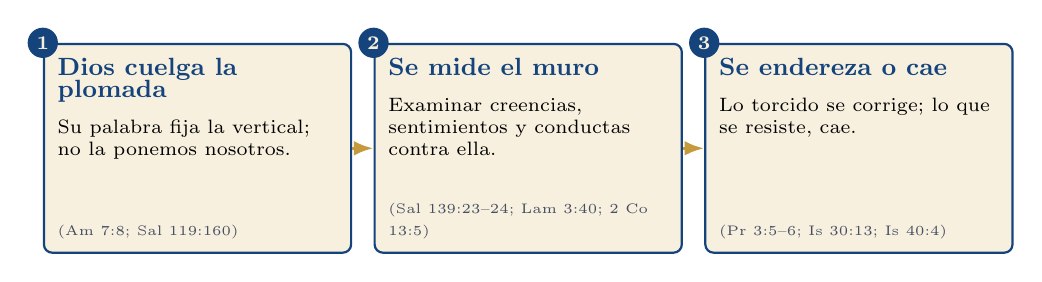
\begin{tikzpicture}
 \foreach \x/\n/\t/\d/\r in {0/1/{Dios cuelga la plomada}/{Su palabra fija la vertical; no la ponemos nosotros.}/{Am 7:8; Sal 119:160},
   4.2/2/{Se mide el muro}/{Examinar creencias, sentimientos y conductas contra ella.}/{Sal 139:23--24; Lam 3:40; 2 Co 13:5},
   8.4/3/{Se endereza o cae}/{Lo torcido se corrige; lo que se resiste, cae.}/{Pr 3:5--6; Is 30:13; Is 40:4}}{
  \node[caja,anchor=north] (b\n) at (\x,0) {\parbox[t][2.3cm][t]{3.55cm}{\RaggedRight
    {\small\textbf{\textcolor{azul}{\t}}}\\[5pt]\scriptsize \d\par\vfill{\tiny\color{gris}(\r)}}};
  \node[circle,fill=azul,text=papiro,font=\scriptsize\bfseries,inner sep=1.6pt] at (b\n.north west) {\n};}
 \draw[-{Latex[length=2.5mm]},dorado,line width=1.2pt] (b1.east) -- (b2.west);
 \draw[-{Latex[length=2.5mm]},dorado,line width=1.2pt] (b2.east) -- (b3.west);
\end{tikzpicture}\par\medskip
\begin{columns}[t,onlytextwidth]
\begin{column}{0.49\textwidth}
\begin{cita}Fíate de \SENOR{} de todo tu corazón, Y no te apoyes en tu propia prudencia. Reconócelo en todos tus caminos, Y él enderezará tus veredas.\fuente{(Pr 3:5--6, RVR1960)}\end{cita}
\end{column}
\begin{column}{0.49\textwidth}
\begin{cita}a la medida de la estatura de la plenitud de Cristo; para que ya no seamos niños fluctuantes, llevados por doquiera de todo viento de doctrina\ldots{} sino que siguiendo la verdad en amor, crezcamos.\fuente{(Ef 4:13--15, RVR1960)}\end{cita}
\end{column}
\end{columns}
\scriptsize En Pablo, la medida es una Persona: \grc{εἰς μέτρον ἡλικίας τοῦ πληρώματος τοῦ Χριστοῦ}. Cristo es la plomada; la deriva es ``todo viento de doctrina''.
\end{frame}

% ------------------------------------------------------------------
\section{Pink}

\begin{frame}{Teología: Pink y la veracidad de Dios}
\begin{columns}[t,onlytextwidth]
\begin{column}{0.55\textwidth}\small
Pink no dedica un capítulo a la verdad; la trata dentro de \destacar{la fidelidad} (Pink, 2020, cap. 10). Su recorrido:
\begin{enumerate}
\item Es esencial al ser de Dios: ``sin ella no sería Dios''; ser infiel sería negarse a sí mismo (2 Ti 2:13).
\item ``Dios es veraz. La promesa de su Palabra es segura'' (Nm 23:19).
\item La historia lo prueba: Gn 15:13--16 se cumple en Éx 12:41; Is 7:14 en Gá 4:4.
\item Aceptar su fidelidad ``como una verdad divina'' no basta: hay que actuar de acuerdo con ella.
\item En la prueba, descansar en esta verdad silencia la queja y engendra confianza.
\end{enumerate}
\end{column}
\begin{column}{0.43\textwidth}
\begin{cita}Dios no es hombre, para que mienta, Ni hijo de hombre para que se arrepienta. El dijo, ¿y no hará? Habló, ¿y no lo ejecutará?\fuente{(Nm 23:19, RVR1960)}\end{cita}
\begin{center}\heb{לֹא אִישׁ אֵל וִיכַזֵּב}\end{center}
\scriptsize \heb{וִיכַזֵּב}, de \heb{כזב}: ``para que mienta''. Lo dice Balaam, un profeta pagano contratado para maldecir.\par\smallskip
\precision{que Pink trate la veracidad dentro de la fidelidad refleja la raíz hebrea común; la fidelidad tendrá su propio estudio (15).}
\end{column}
\end{columns}
\end{frame}

% ------------------------------------------------------------------
\section{Creación}

\begin{frame}{La ciencia no inventa: descubre}
\begin{columns}[c,onlytextwidth]
\begin{column}{0.50\textwidth}
\begin{cita}El que hizo la tierra con su poder, el que puso en orden el mundo con su saber, y extendió los cielos con su sabiduría.\fuente{(Jer 10:12, RVR1960)}\end{cita}
\begin{cita}Porque las cosas invisibles de él, su eterno poder y deidad, se hacen claramente visibles desde la creación del mundo, siendo entendidas por medio de las cosas hechas.\fuente{(Ro 1:20, RVR1960)}\end{cita}
\end{column}
\begin{column}{0.48\textwidth}\small
\begin{itemize}
\item Toda pregunta sobre ciencia o economía es, en el fondo, una pregunta sobre \destacar{cómo Dios estructuró la realidad}.
\item Cuando la física o las matemáticas descubren un patrón exacto, descubren la verdad del diseño de Dios.
\item Cuando la ingeniería respeta la gravedad, la estructura se mantiene en pie: se somete a la verdad material.
\end{itemize}
\scriptsize En el mismo poema de Jer 10, el Dios verdadero (v. 10) es el que ``puso en orden el mundo'' (\heb{מֵכִין תֵּבֵל}, v. 12): el verbo \emph{kun}, ``establecer firme''.
\end{column}
\end{columns}
\end{frame}

\begin{frame}{Primera ley de la termodinámica}
\begin{columns}[t,onlytextwidth]
\begin{column}{0.50\textwidth}\small
\textbf{El postulado.} La energía no se crea ni se destruye: solo se transforma. El universo tiene una cantidad finita de energía que cambia de estado.\par\medskip
\textbf{La correspondencia.} La creación de la nada es un acto exclusivo de Dios que ya concluyó: ``acabó Dios en el día séptimo la obra que hizo'' (Gn 2:2). El universo no genera existencia nueva por sí mismo.
\end{column}
\begin{column}{0.48\textwidth}
\begin{cita}y el polvo vuelva a la tierra, como era, y el espíritu vuelva a Dios que lo dio.\fuente{(Ec 12:7, RVR1960)}\end{cita}
\begin{center}\heb{וְהָרוּחַ תָּשׁוּב אֶל־הָאֱלֹהִים אֲשֶׁר נְתָנָהּ}\end{center}
\scriptsize\heb{רוּחַ} (\emph{rúaj}): aliento, viento, espíritu. En la muerte nada vuelve a la nada: el cuerpo se degrada y el espíritu vuelve a su fuente.\par\smallskip
\precision{la correspondencia es una analogía de tu material: el \emph{rúaj} no es energía física, pero la ley ilustra que la creación no se aniquila ni se crea a sí misma.}
\end{column}
\end{columns}
\end{frame}

\begin{frame}{Segunda ley: la entropía}
\begin{columns}[t,onlytextwidth]
\begin{column}{0.50\textwidth}
\begin{cita}Porque la creación fue sujetada a vanidad, no por su propia voluntad, sino por causa del que la sujetó en esperanza; porque también la creación misma será libertada de la esclavitud de corrupción.\fuente{(Ro 8:20--21, RVR1960)}\end{cita}
\begin{cita}Ellos perecerán, mas tú permanecerás; Y todos ellos como una vestidura se envejecerán.\fuente{(Sal 102:26 [102:27], RVR1960)}\end{cita}
\end{column}
\begin{column}{0.48\textwidth}
\scriptsize\renewcommand{\arraystretch}{1.15}
\begin{tabular}{@{}>{\RaggedRight\arraybackslash}p{2.3cm}>{\RaggedRight\arraybackslash}p{3.0cm}@{}}
\toprule
\textbf{La ciencia} & \textbf{La Biblia} \\ \midrule
la energía útil se disipa & ``como una vestidura se envejecerán'' \\
el desorden aumenta & \grc{ματαιότης}, ``vanidad, frustración'' \\
``aumento de entropía'' & \grc{δουλεία τῆς φθορᾶς}, ``esclavitud de corrupción'' \\
\bottomrule
\end{tabular}\par\medskip
\small El salmista describe un universo que se gasta como ropa vieja; el Creador permanece (He 1:10--12 lo aplica a Cristo).\par\smallskip
\precision{identificar la entropía con la Caída es la lectura de tu material; otros intérpretes ven la segunda ley ya en la creación buena y leen Ro 8:20 como la frustración que siguió al pecado, sin hacerla una ley física.}
\end{column}
\end{columns}
\end{frame}

\begin{frame}{Gobierno, política y economía}
\begin{columns}[t,onlytextwidth]
\begin{column}{0.50\textwidth}
\begin{cita}Y los bendijo Dios, y les dijo: Fructificad y multiplicaos; llenad la tierra, y sojuzgadla, y señoread en los peces del mar\ldots\fuente{(Gn 1:28, RVR1960)}\end{cita}
\scriptsize\renewcommand{\arraystretch}{1.12}
\begin{tabular}{@{}>{\RaggedRight\arraybackslash}p{1.9cm}>{\RaggedRight\arraybackslash}p{4.0cm}@{}}
\toprule
\heb{וְכִבְשֻׁהָ} \emph{kivshuha} & ``y sojuzgadla'': poner bajo orden \\
\heb{וּרְדוּ} \emph{uredú} & ``y señoread'': gobernar como rey \\
\bottomrule
\end{tabular}\par\smallskip
``Cada pregunta sobre política y economía es una pregunta sobre lo que significa ser hecho a la imagen de Dios y tener dominio sobre la Tierra'' (M. Núñez).
\end{column}
\begin{column}{0.48\textwidth}
\begin{tcolorbox}[colback=papiro,colframe=azul,boxrule=0.8pt,arc=3pt,fonttitle=\bfseries\scriptsize,title=Ciencias políticas]
\scriptsize No la búsqueda del poder, sino el diseño de leyes y estructuras que reflejen la justicia y el orden del Creador y protejan a los portadores de su imagen.
\end{tcolorbox}
\begin{tcolorbox}[colback=papiro,colframe=azul,boxrule=0.8pt,arc=3pt,fonttitle=\bfseries\scriptsize,title=Economía]
\scriptsize La mayordomía fiel de los recursos de la creación: organiza el trabajo, la producción y la distribución para el florecimiento humano, frente a la avaricia y el control opresivo.
\end{tcolorbox}
\precision{la cita de Núñez viene de tu material (una predicación); falta la fuente exacta. El mandato es anterior a la Caída (Gn 2:15).}
\end{column}
\end{columns}
\end{frame}

\begin{frame}{El fundamento de la moral}
\begin{columns}[c,onlytextwidth]
\begin{column}{0.52\textwidth}
\begin{tcolorbox}[colback=papiro,colframe=dorado,boxrule=1.2pt,arc=3pt]
\centering\small ``Por encima de los 8000 metros no es un lugar donde la gente pueda permitirse la moralidad.''
\end{tcolorbox}
\scriptsize Palabras de un alpinista japonés en el Everest (1996), después de pasar junto a escaladores agonizantes sin ayudarlos (Krakauer, 1997).\par\medskip
\small Sin la plomada de Dios, el hombre relativiza la moral a su conveniencia y se vuelve capaz de ignorar al caído, y de justificarlo.
\end{column}
\begin{column}{0.46\textwidth}
\begin{cita}Salva, oh \SENOR{}, porque se acabaron los piadosos; Porque han desaparecido los fieles de entre los hijos de los hombres. Habla mentira cada uno con su prójimo.\fuente{(Sal 12:1--2 [12:2--3], RVR1960)}\end{cita}
\scriptsize ``Los fieles'' (\heb{אֱמוּנִים}, \emph{emunim}) son los que viven en \emph{emuná}: cuando desaparecen, desaparece la verdad entre prójimos.\par\smallskip
\precision{la cita se atribuye a un miembro de la expedición de Fukuoka; conviene verificar la página en la edición de Krakauer que uses.}
\end{column}
\end{columns}
\end{frame}

% ------------------------------------------------------------------
\section{Percepción}

\begin{frame}{``Todo hombre es mentiroso''}
\begin{columns}[t,onlytextwidth]
\begin{column}{0.49\textwidth}
\begin{cita}Y dije en mi apresuramiento: Todo hombre es mentiroso.\fuente{(Sal 116:11, RVR1960)}\end{cita}
\begin{center}\heb{כָּל־הָאָדָם כֹּזֵב}\end{center}
\small A causa de la Caída, el ser humano distorsiona la realidad para justificar sus actos o porque interpreta los hechos con límites.
\end{column}
\begin{column}{0.49\textwidth}
\begin{cita}De ninguna manera; antes bien sea Dios veraz, y todo hombre mentiroso.\fuente{(Ro 3:4, RVR1960)}\end{cita}
\scriptsize\renewcommand{\arraystretch}{1.12}
\begin{tabular}{@{}>{\RaggedRight\arraybackslash}p{1.2cm}>{\RaggedRight\arraybackslash}p{4.4cm}@{}}
\toprule
TM & \heb{כָּל־הָאָדָם כֹּזֵב} \\
LXX & \grc{πᾶς ἄνθρωπος ψεύστης} (Sal 115:2) \\
Ro 3:4 & \grc{γινέσθω δὲ ὁ θεὸς ἀληθής, πᾶς δὲ ἄνθρωπος ψεύστης} \\
\bottomrule
\end{tabular}\par\smallskip
Pablo toma el Salmo de la LXX y le antepone la otra mitad: frente al hombre mentiroso, \destacar{Dios veraz}.
\end{column}
\end{columns}
\end{frame}

\begin{frame}{Llamar a lo malo bueno}
\begin{columns}[t,onlytextwidth]
\begin{column}{0.49\textwidth}
\begin{cita}¡Ay de los que a lo malo dicen bueno, y a lo bueno malo; que hacen de la luz tinieblas, y de las tinieblas luz; que ponen lo amargo por dulce, y lo dulce por amargo!\fuente{(Is 5:20, RVR1960)}\end{cita}
\scriptsize\heb{הוֹי הָאֹמְרִים לָרַע טוֹב}: el ``¡ay!'' (\emph{hoy}) de los funerales. Cambiar el nombre de las cosas no cambia las cosas.
\end{column}
\begin{column}{0.49\textwidth}
\begin{cita}Entonces dijo el profeta Jeremías al profeta Hananías: Ahora oye, Hananías: \SENOR{} no te envió, y tú has hecho confiar en mentira a este pueblo.\fuente{(Jer 28:15, RVR1960)}\end{cita}
\scriptsize\heb{הִבְטַחְתָּ}\ldots{} \heb{עַל־שָׁקֶר}: ``hiciste confiar en \emph{shéqer}''. Hananías anunció lo que el pueblo quería oír: paz en dos años (28:3). La mentira cómoda se cree con facilidad; la verdad se reconoce porque se cumple (Dt 18:22; Jer 28:9, 17).
\end{column}
\end{columns}
\end{frame}

\begin{frame}{Sentimientos y realidad biológica}
\begin{columns}[c,onlytextwidth]
\begin{column}{0.52\textwidth}\small
\begin{itemize}
\item Tu material critica la idea de que ``la verdad es lo que yo siento''. Si lo que alguien siente no corresponde con su realidad biológica, ese sentimiento no es verdad.
\item El caso más discutido hoy es la \destacar{identidad sexual}. Marcadores de la realidad: el código genético (XX / XY), el sistema hormonal, la estructura ósea y la cerebral.
\end{itemize}
\scriptsize Núñez (2020, cap. 10): ``Por primera vez en la historia podemos ver que una verdad, en este caso biológica, es definida en base a un sentimiento\ldots{} Explicar la verdad tal como es, podría ayudar más a estas personas a aceptar su realidad que mutilar su cuerpo para adaptarlo a una irrealidad de la mente''.
\end{column}
\begin{column}{0.46\textwidth}
\begin{tcolorbox}[colback=papiro,colframe=dorado,boxrule=1.2pt,arc=3pt]
\small\itshape ``No es tu cuerpo el que tenemos que ajustar con cirugías, es tu mente la que tenemos que ajustar con la verdad y llevarla a la verticalidad de la verdad de Dios.''\par\smallskip\upshape\hfill\scriptsize M. Núñez
\end{tcolorbox}
\begin{cita}Varón y hembra los creó.\fuente{(Gn 1:27, RVR1960)}\end{cita}
\precision{la cita en el recuadro viene de tu material (predicación); falta la fuente exacta. La del libro de Núñez se cita desde la biblioteca de la serie.}
\end{column}
\end{columns}
\end{frame}

\begin{frame}{Documentación clínica y legal}
\centering
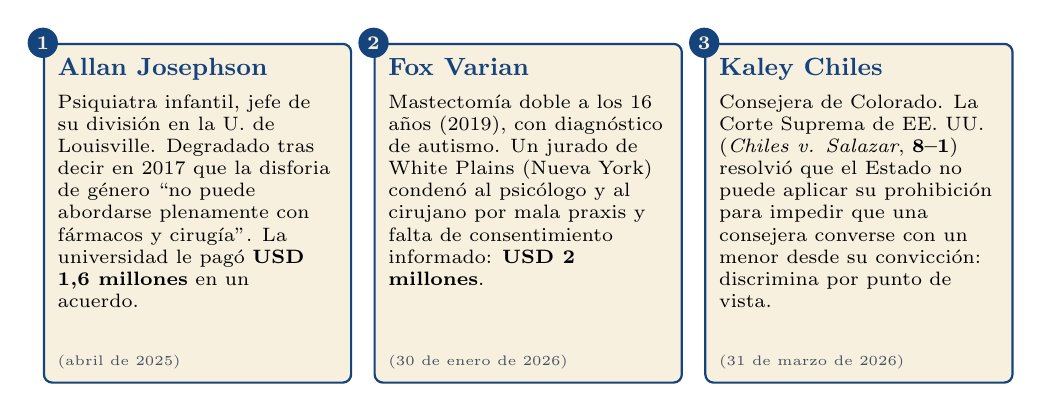
\begin{tikzpicture}
 \foreach \x/\n/\t/\d/\r in {0/1/{Allan Josephson}/{Psiquiatra infantil, jefe de su división en la U. de Louisville. Degradado tras decir en 2017 que la disforia de género ``no puede abordarse plenamente con fármacos y cirugía''. La universidad le pagó \textbf{USD 1,6 millones} en un acuerdo.}/{abril de 2025},
   4.2/2/{Fox Varian}/{Mastectomía doble a los 16 años (2019), con diagnóstico de autismo. Un jurado de White Plains (Nueva York) condenó al psicólogo y al cirujano por mala praxis y falta de consentimiento informado: \textbf{USD 2 millones}.}/{30 de enero de 2026},
   8.4/3/{Kaley Chiles}/{Consejera de Colorado. La Corte Suprema de EE.~UU. (\emph{Chiles v. Salazar}, \textbf{8--1}) resolvió que el Estado no puede aplicar su prohibición para impedir que una consejera converse con un menor desde su convicción: discrimina por punto de vista.}/{31 de marzo de 2026}}{
  \node[caja,anchor=north] (b\n) at (\x,0) {\parbox[t][3.95cm][t]{3.55cm}{\RaggedRight
    {\small\textbf{\textcolor{azul}{\t}}}\\[4pt]\scriptsize \d\par\vfill{\tiny\color{gris}(\r)}}};
  \node[circle,fill=azul,text=papiro,font=\scriptsize\bfseries,inner sep=1.6pt] at (b\n.north west) {\n};}
\end{tikzpicture}\par\medskip
\small\RaggedRight Alterar la biología para acomodar una percepción genera estragos; tres casos recientes en EE.~UU. llegaron a tribunales.
\end{frame}

\begin{frame}{Qué dicen y qué no dicen los tres casos}
\scriptsize\renewcommand{\arraystretch}{1.22}
\begin{tabular}{@{}>{\RaggedRight\arraybackslash}p{2.0cm}>{\RaggedRight\arraybackslash}p{4.9cm}>{\RaggedRight\arraybackslash}p{4.9cm}@{}}
\toprule
\textbf{Caso} & \textbf{Lo que se resolvió} & \textbf{Precisión frente al material} \\ \midrule
Josephson & El Sexto Circuito (2024) permitió que la demanda fuera a juicio; la universidad pagó antes del juicio. & No hubo sentencia sobre el fondo: fue un acuerdo, no una corte que ``validó'' su postura clínica. \\
Varian & Veredicto de jurado por mala praxis: USD 1,6 millones por daño y 0,4 por gastos médicos futuros. & El jurado juzgó el estándar de cuidado y el consentimiento, no la ideología; la fecha es 30 de enero (se informó en febrero). \\
Chiles & La ley de Colorado no puede aplicarse a la conversación terapéutica de Chiles; debe pasar el escrutinio más estricto de la Primera Enmienda. & Es un fallo sobre libertad de expresión. La ley prohibía ayudar a cambiar la orientación o identidad de un menor; no obligaba a ``afirmar''. \\
\bottomrule
\end{tabular}\par\medskip
\precision{fuentes periodísticas y jurídicas: Spectrum News (21-04-2025); ABA Journal (04-02-2026) y ADF; opinión de la Corte Suprema, \emph{Chiles v. Salazar} (31-03-2026). Conviene presentarlos como hechos documentados, sin agregar lo que los fallos no dicen.}
\end{frame}

% ------------------------------------------------------------------
\section{En Israel}

\begin{frame}{Un encuentro: la viuda de Sarepta}
\begin{columns}[t,onlytextwidth]
\begin{column}{0.54\textwidth}
\begin{cita}Y se tendió sobre el niño tres veces, y clamó a \SENOR{} y dijo: \SENOR{} Dios mío, te ruego que hagas volver el alma de este niño a él. Y \SENOR{} oyó la voz de Elías, y el alma del niño volvió a él, y revivió. Tomando luego Elías al niño, lo trajo del aposento a la casa, y lo dio a su madre, y le dijo Elías: Mira, tu hijo vive. Entonces la mujer dijo a Elías: Ahora conozco que tú eres varón de Dios, y que la palabra de \SENOR{} es verdad en tu boca.\fuente{(1~R 17:21--24, RVR1960)}\end{cita}
\begin{center}\heb{וּדְבַר־יְהוָה בְּפִיךָ אֱמֶת}\end{center}
\end{column}
\begin{column}{0.44\textwidth}\small
\begin{itemize}
\item Sarepta estaba en Sidón, tierra de Baal, el dios de la lluvia. Elías había anunciado: ``no habrá lluvia ni rocío'' (17:1).
\item La palabra ya se había cumplido una vez: la harina y el aceite ``conforme a la palabra'' (17:16).
\item Ella ya lo llamaba ``varón de Dios'' (17:18); ahora \destacar{conoce}: la palabra es \emph{emet} porque da vida.
\end{itemize}
\end{column}
\end{columns}
\end{frame}

\begin{frame}{De Sarepta al Carmelo, y a Naín}
\centering
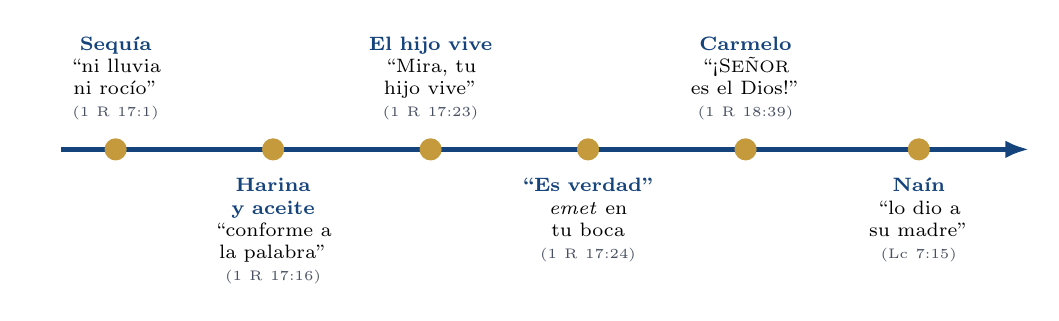
\begin{tikzpicture}[font=\scriptsize]
 \draw[line width=1.6pt,azul,-{Latex[length=3mm]}] (-0.3,0) -- (12.0,0);
 \foreach \x/\t/\b/\r/\pos in {0.4/{Sequía}/{``ni lluvia ni rocío''}/{1~R 17:1}/above,
   2.4/{Harina y aceite}/{``conforme a la palabra''}/{1~R 17:16}/below,
   4.4/{El hijo vive}/{``Mira, tu hijo vive''}/{1~R 17:23}/above,
   6.4/{``Es verdad''}/{\emph{emet} en tu boca}/{1~R 17:24}/below,
   8.4/{Carmelo}/{``¡\SENOR{} es el Dios!''}/{1~R 18:39}/above,
   10.6/{Naín}/{``lo dio a su madre''}/{Lc 7:15}/below}{
  \fill[dorado] (\x,0) circle (4pt);
  \node[\pos=7pt,text width=2.0cm,align=center] at (\x,0) {\textbf{\textcolor{azul}{\t}}\\ \b\\ {\tiny\color{gris}(\r)}};}
\end{tikzpicture}\par\medskip
\begin{columns}[t,onlytextwidth]
\begin{column}{0.49\textwidth}\small
La verdad de Dios no se demuestra con un argumento, sino con \destacar{vida}: el Dios verdadero es el ``Dios vivo'' (Jer 10:10). Baal no pudo dar lluvia; el \SENOR{} devolvió un hijo.
\end{column}
\begin{column}{0.49\textwidth}\scriptsize
Jesús recuerda a esta viuda en Nazaret (Lc 4:25--26). En Naín resucita al hijo de otra viuda, y Lucas usa las palabras de la LXX: \grc{καὶ ἔδωκεν αὐτὸν τῇ μητρὶ αὐτοῦ} (Lc 7:15 = 1~R 17:23 LXX).\par\smallskip
\precision{el eco verbal está en el texto griego; la conexión con Jer 10:10 es propia de esta serie.}
\end{column}
\end{columns}
\end{frame}

% ------------------------------------------------------------------
\section{Judaísmo}

\begin{frame}{``El sello del Santo es \emph{emet}''}
\begin{columns}[t,onlytextwidth]
\begin{column}{0.52\textwidth}\small
\textbf{Talmud de Babilonia} (\emph{Shabat} 55a). Rabí Janiná:
\begin{center}\heb{חוֹתָמוֹ שֶׁל הַקָּדוֹשׁ בָּרוּךְ הוּא אֱמֶת}\end{center}
``El sello del Santo, bendito sea, es \emph{emet}''.\par\medskip
\textbf{Talmud de Jerusalén} (\emph{Sanedrín} 1:1). Ante la misma pregunta, Rabí Bun explica qué es \emph{emet}: \heb{שֶׁהוּא אֱלֹהִים חַיִּים וּמֶלֶךְ עוֹלָם}, ``que él es Dios vivo y Rey eterno'': las palabras de \destacar{Jer 10:10}.
\end{column}
\begin{column}{0.46\textwidth}
\centering
\begin{tikzpicture}[font=\scriptsize]
 \draw[azul,line width=0.8pt] (-2.6,0) -- (2.6,0);
 \foreach \x/\l/\t in {2.4/{א}/{la primera},0/{מ}/{la del medio},-2.4/{ת}/{la última}}{
  \node[draw=dorado,line width=1.3pt,fill=azul,text=papiro,circle,minimum size=0.95cm,font=\Large] at (\x,0) {\heb{\l}};
  \node[below=12pt,font=\tiny,text=gris] at (\x,0) {\t};}
\end{tikzpicture}\par\smallskip
\scriptsize Resh Laquish: álef abre el alfabeto, mem está en el medio y tav lo cierra. Dios es el primero, que no recibió de otro, y el último, que no entregará a otro (Is 41:4; cf. 44:6).\par\smallskip
\precision{interpretación rabínica; texto según Sefaria (edición William Davidson y Talmud de Jerusalén, ed. Guggenheimer).}
\end{column}
\end{columns}
\end{frame}

\begin{frame}{La verdad tiene pies anchos}
\begin{columns}[c,onlytextwidth]
\begin{column}{0.50\textwidth}
\centering
\begin{tikzpicture}
 \node[font=\fontsize{40}{40}\selectfont,text=azul] (e) at (0,1.3) {\heb{אמת}};
 \node[font=\scriptsize\bfseries,text=azul,text width=4.5cm,align=center] at (0,0.35) {\emph{emet}: letras separadas en el alfabeto, de base ancha};
 \node[font=\fontsize{40}{40}\selectfont,text=gris] (s) at (0,-1.0) {\heb{שקר}};
 \node[font=\scriptsize\bfseries,text=gris,text width=4.5cm,align=center] at (0,-1.95) {\emph{shéqer}: letras vecinas, apoyadas en una punta};
\end{tikzpicture}
\end{column}
\begin{column}{0.48\textwidth}\small
\textbf{\emph{Shabat} 104a.} Las letras de \emph{shéqer} (\heb{ש ק ר}) están juntas en el alfabeto; las de \emph{emet} (\heb{א מ ת}), lejos: la mentira es común y la verdad escasa. Además, las letras de \emph{shéqer} se apoyan en un solo pie; las de \emph{emet}, en una base firme:
\begin{center}\heb{קוּשְׁטָא קָאֵי שִׁיקְרָא לָא קָאֵי}\end{center}
``La verdad se mantiene en pie; la mentira no se mantiene''.
\end{column}
\end{columns}\par\medskip
\precision{interpretación rabínica sobre la forma de las letras. Es la ``plomada'' de tu material dicha por los sabios: la verdad queda en pie (cf. Pr 12:19).}
\end{frame}

\begin{frame}{La verdad arrojada a la tierra}
\begin{columns}[t,onlytextwidth]
\begin{column}{0.52\textwidth}\small
\textbf{\emph{Bereshit Rabá} 8:5.} Rabí Simón: cuando Dios iba a crear al hombre, los ángeles se dividieron. La Misericordia dijo ``que sea creado'', porque hará actos de bondad; la Verdad dijo ``que no sea creado'', \heb{שֶׁכֻּלּוֹ שְׁקָרִים}, ``porque todo él es mentiras''. ¿Qué hizo el Santo? \heb{נָטַל אֱמֶת וְהִשְׁלִיכוֹ לָאָרֶץ}: ``tomó la verdad y la arrojó a la tierra'' (Dn 8:12). Y citan:
\begin{center}\heb{אֱמֶת מֵאֶרֶץ תִּצְמָח}\end{center}
\end{column}
\begin{column}{0.46\textwidth}
\begin{cita}La misericordia y la verdad se encontraron; La justicia y la paz se besaron. La verdad brotará de la tierra, Y la justicia mirará desde los cielos.\fuente{(Sal 85:10--11 [85:11--12], RVR1960)}\end{cita}
\precision{interpretación rabínica (midrash). Leer en Cristo ``la verdad que brota de la tierra'' (Jn 1:14) es una lectura cristiana tradicional, no del midrash.}
\end{column}
\end{columns}
\end{frame}

\begin{frame}{La verdad en la oración y en la Misná}
\scriptsize\renewcommand{\arraystretch}{1.2}
\begin{tabular}{@{}>{\RaggedRight\arraybackslash}p{2.6cm}>{\RaggedRight\arraybackslash}p{9.2cm}@{}}
\toprule
\textbf{\emph{Berajot} 14b} & Al terminar el \emph{Shemá} con ``Yo soy el \SENOR{} vuestro Dios'' (Nm 15:41), se agrega en seguida \emph{emet}, ``verdad'', por Jer 10:10: \heb{וַיהוָה אֱלֹהִים אֱמֶת}. Así, en la oración diaria, el Nombre y la verdad no se separan. \\
\textbf{\emph{Emet veyatsiv}} & la bendición de la mañana que sigue al \emph{Shemá} comienza \heb{אֱמֶת וְיַצִּיב}, ``verdadero y firme'', y la de la tarde \heb{אֱמֶת וֶאֱמוּנָה}, ``verdad y fidelidad'' (Elbogen, 1993). \\
\textbf{\emph{Avot} 1:18} & Rabán Shimón ben Gamliel: \heb{עַל שְׁלֹשָׁה דְבָרִים הָעוֹלָם עוֹמֵד} ``sobre tres cosas se sostiene el mundo: la justicia, la verdad y la paz'', y cita Zac 8:16. \\
\textbf{Maimónides} & \emph{Mishné Torá}, \emph{Yesodé haTorá} 1:4, cita Jer 10:10: \heb{הוּא לְבַדּוֹ הָאֱמֶת}, ``él solo es la verdad, y ningún otro tiene verdad como la suya''. \\
\bottomrule
\end{tabular}\par\medskip
\begin{cita}Hablad verdad cada cual con su prójimo; juzgad según la verdad y lo conducente a la paz en vuestras puertas.\fuente{(Zac 8:16, RVR1960)}\end{cita}
\precision{interpretaciones y usos litúrgicos judíos, según Sefaria. Tres de las cuatro fuentes se apoyan en el texto ancla de este estudio.}
\end{frame}

\begin{frame}{Qumrán: el espíritu de verdad}
\begin{columns}[t,onlytextwidth]
\begin{column}{0.52\textwidth}\small
La \emph{Regla de la Comunidad} (1QS) describe dos espíritus que Dios dio al hombre:
\begin{center}\heb{רוּחוֹת הָאֱמֶת וְהָעָוֶל}\end{center}
``los espíritus de la verdad y de la perversidad'' (1QS 3:18--19). Los ``hijos de la verdad'' andan en la luz; los de la perversidad, en tinieblas.\par\smallskip
\scriptsize Al fin, Dios ``rociará sobre él el espíritu de verdad como aguas de purificación'' (1QS 4:21), lenguaje de Ez 36:25--27. Y el ingreso a la comunidad es para ``practicar la verdad, la justicia y el derecho en la tierra'' (1QS 1:5), eco de Jer 9:24.
\end{column}
\begin{column}{0.46\textwidth}
\begin{cita}el Espíritu de verdad, al cual el mundo no puede recibir, porque no le ve, ni le conoce.\fuente{(Jn 14:17, RVR1960)}\end{cita}
\begin{cita}Mas el que practica la verdad viene a la luz.\fuente{(Jn 3:21, RVR1960)}\end{cita}
\precision{traducción según García Martínez (1992) y Vermes (2004); cotejar las imágenes de 1QS en la Leon Levy Dead Sea Scrolls Digital Library. Los paralelos con Juan los señalan los estudios del NT; no implican dependencia directa.}
\end{column}
\end{columns}
\end{frame}

% ------------------------------------------------------------------
\section{En Cristo}

\begin{frame}{Cambiaron la verdad por la mentira}
\begin{columns}[t,onlytextwidth]
\begin{column}{0.50\textwidth}
\begin{cita}Porque la ira de Dios se revela desde el cielo contra toda impiedad e injusticia de los hombres que detienen con injusticia la verdad\ldots{} ya que cambiaron la verdad de Dios por la mentira, honrando y dando culto a las criaturas antes que al Creador.\fuente{(Ro 1:18, 25, RVR1960)}\end{cita}
\end{column}
\begin{column}{0.48\textwidth}
\scriptsize\renewcommand{\arraystretch}{1.15}
\begin{tabular}{@{}>{\RaggedRight\arraybackslash}p{1.7cm}>{\RaggedRight\arraybackslash}p{3.7cm}@{}}
\toprule
Ro 1:18 & \grc{τὴν ἀλήθειαν ἐν ἀδικίᾳ κατεχόντων}: ``reteniendo, sujetando la verdad'' \\
Ro 1:25 & \grc{μετήλλαξαν τὴν ἀλήθειαν τοῦ θεοῦ ἐν τῷ ψεύδει}: ``trocaron la verdad de Dios por \emph{la} mentira'' \\
Jer 10:14 & \heb{כִּי שֶׁקֶר נִסְכּוֹ}; LXX \grc{ψευδῆ ἐχώνευσαν}, ``fundieron mentiras'' \\
\bottomrule
\end{tabular}\par\medskip
\small Para Pablo, ``la mentira'' (con artículo) es el \destacar{ídolo}: el mismo juicio de Jeremías. La verdad de Dios es Dios mismo, conocido por lo creado (1:20).
\end{column}
\end{columns}
\precision{la lectura de ``la mentira'' como la idolatría es común en los comentaristas (Moo, 1996); el vínculo con Jer 10:14 es de esta serie.}
\end{frame}

\begin{frame}{``Sea Dios veraz''}
\begin{columns}[t,onlytextwidth]
\begin{column}{0.50\textwidth}
\begin{cita}¿Pues qué, si algunos de ellos han sido incrédulos? ¿Su incredulidad habrá hecho nula la fidelidad de Dios? De ninguna manera; antes bien sea Dios veraz, y todo hombre mentiroso.\fuente{(Ro 3:3--4, RVR1960)}\end{cita}
\end{column}
\begin{column}{0.48\textwidth}\small
\begin{itemize}
\item \grc{ἀπιστία} (incredulidad) frente a \grc{πίστις τοῦ θεοῦ} (fidelidad de Dios): el par hebreo \emph{emuná}.
\item \grc{ἀληθής}: Dios es veraz porque \destacar{cumple} lo que prometió a Israel aunque Israel falle.
\item En 3:7 Pablo habla de ``la verdad de Dios'' (\grc{ἡ ἀλήθεια τοῦ θεοῦ}) como sinónimo de su fidelidad.
\end{itemize}
\end{column}
\end{columns}\par\smallskip
\precision{Pablo une las dos caras de la raíz \emph{amán}: fidelidad (3:3) y verdad (3:4, 7). Es la teología de Sal 116:11 y de Nm 23:19 leída en Romanos.}
\end{frame}

\begin{frame}{Cristo, siervo de la verdad de Dios}
\begin{columns}[t,onlytextwidth]
\begin{column}{0.50\textwidth}
\begin{cita}Pues os digo, que Cristo Jesús vino a ser siervo de la circuncisión para mostrar la verdad de Dios, para confirmar las promesas hechas a los padres, y para que los gentiles glorifiquen a Dios por su misericordia.\fuente{(Ro 15:8--9, RVR1960)}\end{cita}
\scriptsize\grc{ὑπὲρ ἀληθείας θεοῦ, εἰς τὸ βεβαιῶσαι τὰς ἐπαγγελίας}: ``a favor de la verdad de Dios, para confirmar (hacer firmes) las promesas''.
\end{column}
\begin{column}{0.48\textwidth}
\begin{cita}Cumplirás la verdad a Jacob, y a Abraham la misericordia, que juraste a nuestros padres desde tiempos antiguos.\fuente{(Mi 7:20, RVR1960)}\end{cita}
\small Miqueas pide \emph{emet} para Jacob y \emph{jésed} para Abraham; Pablo dice que Cristo trajo la \destacar{verdad} a Israel y la \destacar{misericordia} a las naciones. \grc{βεβαιόω} es casi una traducción de \emph{amán}: afirmar.
\end{column}
\end{columns}
\end{frame}

\begin{frame}{``En él Sí, y en él Amén''}
\fotolado{panel_2corintios1.jpg}{Elaboración propia: 2 Co 1:20 en escritura uncial (texto NA28).}
\begin{columns}[c,onlytextwidth]
\begin{column}{0.58\textwidth}
\begin{cita}Mas, como Dios es fiel, nuestra palabra a vosotros no es Sí y No. Porque el Hijo de Dios, Jesucristo\ldots{} no ha sido Sí y No; mas ha sido Sí en él; porque todas las promesas de Dios son en él Sí, y en él Amén, por medio de nosotros, para la gloria de Dios.\fuente{(2~Co 1:18--20, RVR1960)}\end{cita}
\centering
\begin{tikzpicture}[font=\scriptsize,node distance=0.35cm]
 \node[caja,text width=1.9cm,align=center] (a) {Is 65:16\\ \emph{Elohé amén}};
 \node[caja,text width=1.9cm,align=center,right=of a] (b) {2 Co 1:20\\ \grc{τὸ ἀμήν}};
 \node[draw=dorado,line width=1.3pt,fill=azul,text=papiro,rounded corners=3pt,text width=1.9cm,align=center,inner sep=4pt,right=of b] (c) {Ap 3:14\\ ``el Amén''};
 \draw[-{Latex[length=2mm]},dorado,line width=1pt](a)--(b); \draw[-{Latex[length=2mm]},dorado,line width=1pt](b)--(c);
\end{tikzpicture}
\end{column}
\begin{column}{0.40\textwidth}\end{column}
\end{columns}
\end{frame}

\begin{frame}{El Dios vivo y verdadero}
\begin{columns}[t,onlytextwidth]
\begin{column}{0.50\textwidth}
\begin{cita}y cómo os convertisteis de los ídolos a Dios, para servir al Dios vivo y verdadero, y esperar de los cielos a su Hijo, al cual resucitó de los muertos.\fuente{(1~Ts 1:9--10, RVR1960)}\end{cita}
\scriptsize\renewcommand{\arraystretch}{1.12}
\begin{tabular}{@{}>{\RaggedRight\arraybackslash}p{1.4cm}>{\RaggedRight\arraybackslash}p{4.6cm}@{}}
\toprule
Jer 10:10 & \heb{אֱלֹהִים אֱמֶת}\ldots{} \heb{אֱלֹהִים חַיִּים} \\
1 Ts 1:9 & \grc{θεῷ ζῶντι καὶ ἀληθινῷ} \\
\bottomrule
\end{tabular}
\end{column}
\begin{column}{0.48\textwidth}\small
\begin{itemize}
\item Es probablemente la carta más antigua de Pablo. Resume su predicación a gentiles con el lenguaje de Jer 10: \destacar{dejar los ídolos} por el Dios vivo y verdadero.
\item La prueba de que Dios es ``vivo'' es que \destacar{resucitó} a su Hijo: lo que en Sarepta fue un anticipo.
\end{itemize}
\precision{Jer 10:10 falta en la LXX; Pablo usa una fórmula judía corriente (cf. Is 65:16 LXX, \grc{θεὸν ἀληθινόν}). El eco de Jer 10 es probable, no seguro.}
\end{column}
\end{columns}
\end{frame}

\begin{frame}{La verdad está en Jesús}
\centering
\begin{tikzpicture}[font=\scriptsize]
 \node[caja,text width=4.4cm,align=center] (m) at (-3.0,1.25) {\textbf{Jer 10:10; Éx 34:6}\\ ``Dios verdad''; ``grande en misericordia y verdad''};
 \node[caja,text width=4.4cm,align=center] (j) at (3.0,1.25) {\textbf{Jn 1:14, 17; 14:6}\\ ``lleno de gracia y de verdad''; ``yo soy\ldots{} la verdad''};
 \node[draw=dorado,line width=1.6pt,fill=azul,text=papiro,rounded corners=3pt,text width=6.6cm,align=center,inner sep=5pt] (p) at (0,-1.0) {\textbf{Ef 4:21; Col 2:9}\\ ``conforme a la verdad que está en Jesús'' (\grc{καθώς ἐστιν ἀλήθεια ἐν τῷ Ἰησοῦ}); ``en él habita corporalmente toda la plenitud de la Deidad''};
 \draw[-{Latex[length=2.5mm]},dorado,line width=1.2pt] (m)--(p);
 \draw[-{Latex[length=2.5mm]},dorado,line width=1.2pt] (j)--(p);
\end{tikzpicture}\par\medskip
\begin{columns}[t,onlytextwidth]
\begin{column}{0.49\textwidth}
\begin{cita}Jesús le dijo: Yo soy el camino, y la verdad, y la vida; nadie viene al Padre, sino por mí.\fuente{(Jn 14:6, RVR1960)}\end{cita}
\end{column}
\begin{column}{0.49\textwidth}\scriptsize
La revelación culminante del NT es que la verdad no es un simple concepto: es una \destacar{Persona}. Pablo advierte contra ``filosofías y huecas sutilezas\ldots{} y no según Cristo'' (Col 2:8).\par\smallskip
\precision{Juan no es Pablo; la autoría de Efesios y Colosenses se discute, pero Ro 15:8 y 2 Co 1:20 dicen lo mismo en cartas indiscutidas.}
\end{column}
\end{columns}
\end{frame}

\begin{frame}{La piedra de cimiento estable}
\begin{columns}[t,onlytextwidth]
\begin{column}{0.50\textwidth}
\scriptsize\renewcommand{\arraystretch}{1.18}
\begin{tabular}{@{}>{\RaggedRight\arraybackslash}p{1.2cm}>{\RaggedRight\arraybackslash}p{4.8cm}@{}}
\toprule
Is 28:16 TM & \heb{מוּסָד מוּסָּד הַמַּאֲמִין לֹא יָחִישׁ}: ``cimiento bien cimentado; el que cree no se apresurará'' \\
LXX & \grc{ὁ πιστεύων ἐπ' αὐτῷ οὐ μὴ καταισχυνθῇ}: ``no será avergonzado'' \\
Ro 9:33 & piedra de tropiezo; ``el que creyere en él, no será avergonzado'' \\
Ro 10:11 & \grc{πᾶς ὁ πιστεύων ἐπ' αὐτῷ}: ``todo aquel'' \\
\bottomrule
\end{tabular}
\end{column}
\begin{column}{0.48\textwidth}\small
\begin{itemize}
\item En Isaías, Dios pone en Sion una piedra probada y \destacar{mide con plomada} (28:17). Lo que no está a plomo, ``el refugio de la mentira'', se lo lleva el granizo.
\item Pablo identifica la piedra con \destacar{Cristo}: él es lo firme (\emph{emet}) en que se apoya el que cree (\emph{hama'amín}).
\end{itemize}
\end{column}
\end{columns}\par\medskip
\centering
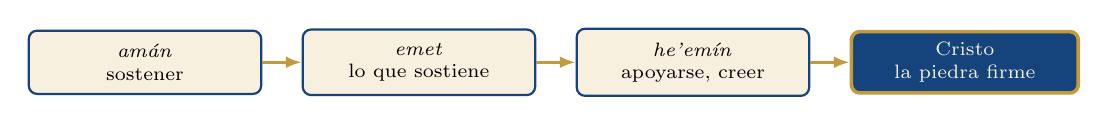
\begin{tikzpicture}[font=\scriptsize,node distance=0.5cm]
 \node[caja,text width=2.6cm,align=center] (a) {\emph{amán}\\ sostener};
 \node[caja,text width=2.6cm,align=center,right=of a] (b) {\emph{emet}\\ lo que sostiene};
 \node[caja,text width=2.6cm,align=center,right=of b] (c) {\emph{he'emín}\\ apoyarse, creer};
 \node[draw=dorado,line width=1.3pt,fill=azul,text=papiro,rounded corners=3pt,text width=2.6cm,align=center,inner sep=4pt,right=of c] (d) {Cristo\\ la piedra firme};
 \foreach \i/\j in {a/b,b/c,c/d}\draw[-{Latex[length=2mm]},dorado,line width=1pt](\i)--(\j);
\end{tikzpicture}
\end{frame}

\begin{frame}{Mentir profana a una Persona}
\begin{columns}[t,onlytextwidth]
\begin{column}{0.50\textwidth}
\begin{cita}Vosotros sois de vuestro padre el diablo, y los deseos de vuestro padre queréis hacer. El ha sido homicida desde el principio, y no ha permanecido en la verdad, porque no hay verdad en él. Cuando habla mentira, de suyo habla; porque es mentiroso, y padre de mentira.\fuente{(Jn 8:44, RVR1960)}\end{cita}
\end{column}
\begin{column}{0.48\textwidth}\small
Si la verdad es una Persona, mentir o aliarse con la falsedad no deshonra solo un concepto ético: \destacar{profana a una Persona} y se alía con el padre de mentira.
\begin{cita}Por lo cual, desechando la mentira, hablad verdad cada uno con su prójimo; porque somos miembros los unos de los otros.\fuente{(Ef 4:25, RVR1960)}\end{cita}
\scriptsize\grc{λαλεῖτε ἀλήθειαν ἕκαστος μετὰ τοῦ πλησίον αὐτοῦ}: cita casi literal de Zac 8:16 LXX. La razón es nueva: \emph{somos miembros} del cuerpo de Cristo.
\end{column}
\end{columns}
\end{frame}

\begin{frame}{La verdad que hace libres}
\begin{columns}[t,onlytextwidth]
\begin{column}{0.49\textwidth}
\begin{cita}Si vosotros permaneciereis en mi palabra, seréis verdaderamente mis discípulos; y conoceréis la verdad, y la verdad os hará libres.\fuente{(Jn 8:31--32, RVR1960)}\end{cita}
\scriptsize\grc{ἡ ἀλήθεια ἐλευθερώσει ὑμᾶς}. La libertad viene de \emph{permanecer} (\grc{μένω}) en su palabra: la firmeza otra vez.
\end{column}
\begin{column}{0.49\textwidth}
\begin{cita}sino por la manifestación de la verdad recomendándonos a toda conciencia humana delante de Dios\ldots{} Porque Dios, que mandó que de las tinieblas resplandeciese la luz, es el que resplandeció en nuestros corazones, para iluminación del conocimiento de la gloria de Dios en la faz de Jesucristo.\fuente{(2~Co 4:2, 6, RVR1960)}\end{cita}
\end{column}
\end{columns}\par\smallskip
\small\RaggedRight Solo sujetos a Cristo, la Verdad encarnada y la plomada del universo, encontramos salvación y libertad. La gloria que Moisés pidió ver (Éx 33:18) tiene rostro.
\end{frame}

% ------------------------------------------------------------------
\section{Vivirlo}

\begin{frame}{Un atributo comunicable}
\begin{columns}[t,onlytextwidth]
\begin{column}{0.49\textwidth}
\begin{cita}\SENOR{}, ¿quién habitará en tu tabernáculo? ¿Quién morará en tu monte santo? El que anda en integridad y hace justicia, Y habla verdad en su corazón.\fuente{(Sal 15:1--2, RVR1960)}\end{cita}
\scriptsize\heb{וְדֹבֵר אֱמֶת בִּלְבָבוֹ}: ``y habla verdad \emph{en} su corazón''. La verdad empieza adentro, antes de llegar a los labios (Sal 51:6).
\end{column}
\begin{column}{0.49\textwidth}\small
\begin{itemize}
\item Como fuente, la verdad es solo de Dios: ``él solo es la verdad'' (Maimónides). Como \destacar{veracidad}, se comunica.
\item ``Siguiendo la verdad en amor'' (\grc{ἀληθεύοντες ἐν ἀγάπῃ}, Ef 4:15): verdad sin amor hiere; amor sin verdad engaña.
\item ``Amad, pues, la verdad y la paz'' (Zac 8:19): \heb{וְהָאֱמֶת וְהַשָּׁלוֹם אֱהָבוּ}.
\end{itemize}
\end{column}
\end{columns}
\end{frame}

\begin{frame}{Cuatro respuestas a la verdad}
\centering
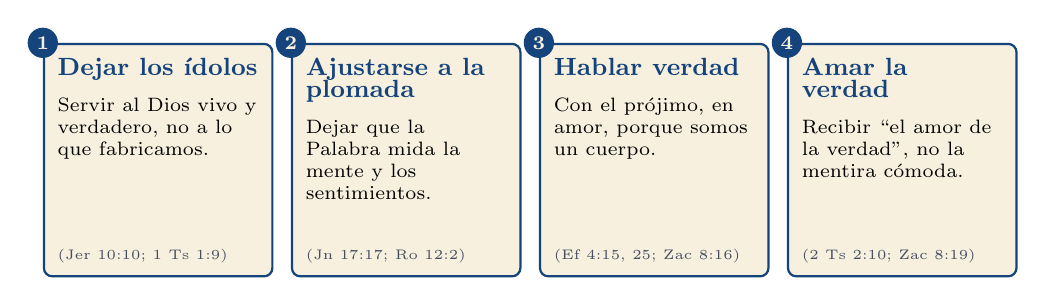
\begin{tikzpicture}
 \foreach \x/\n/\t/\d/\r in {0/1/{Dejar los ídolos}/{Servir al Dios vivo y verdadero, no a lo que fabricamos.}/{Jer 10:10; 1 Ts 1:9},
   3.15/2/{Ajustarse a la plomada}/{Dejar que la Palabra mida la mente y los sentimientos.}/{Jn 17:17; Ro 12:2},
   6.3/3/{Hablar verdad}/{Con el prójimo, en amor, porque somos un cuerpo.}/{Ef 4:15, 25; Zac 8:16},
   9.45/4/{Amar la verdad}/{Recibir ``el amor de la verdad'', no la mentira cómoda.}/{2 Ts 2:10; Zac 8:19}}{
  \node[caja,anchor=north] (b\n) at (\x,0) {\parbox[t][2.6cm][t]{2.55cm}{\RaggedRight
    {\small\textbf{\textcolor{azul}{\t}}}\\[5pt]\scriptsize \d\par\vfill{\tiny\color{gris}(\r)}}};
  \node[circle,fill=azul,text=papiro,font=\scriptsize\bfseries,inner sep=1.6pt] at (b\n.north west) {\n};}
\end{tikzpicture}\par\medskip
\begin{cita}y con todo engaño de iniquidad para los que se pierden, por cuanto no recibieron el amor de la verdad para ser salvos.\fuente{(2~Ts 2:10, RVR1960)}\end{cita}
\scriptsize\grc{τὴν ἀγάπην τῆς ἀληθείας οὐκ ἐδέξαντο}: la verdad no solo se conoce; se \emph{ama}.
\end{frame}

\begin{frame}{Aplicación al corazón}
\begin{tcolorbox}[colback=papiro,colframe=dorado,boxrule=1.4pt,arc=3pt]
\centering\large ¿Estoy dispuesto a ajustar mi mente, mis emociones y mi vida a la plomada de la verdad de Dios, o espero que la verdad se incline a lo que yo siento?
\end{tcolorbox}\par\medskip
\begin{cita}Santifícalos en tu verdad; tu palabra es verdad.\fuente{(Jn 17:17, RVR1960)}\end{cita}
\begin{cita}No os conforméis a este siglo, sino transformaos por medio de la renovación de vuestro entendimiento.\fuente{(Ro 12:2, RVR1960)}\end{cita}
\end{frame}

% ------------------------------------------------------------------
\section{Síntesis}

\begin{frame}{Síntesis}
\begin{tcolorbox}[colback=papiro,colframe=azul,boxrule=1pt,arc=3pt]
\small Frente a ídolos clavados para no caerse, Jeremías confiesa: ``Mas \SENOR{} es el Dios verdadero'' (\emph{Elohim emet}, Jer 10:10). La verdad de Dios es \destacar{firmeza} (raíz \emph{amán}), \destacar{correspondencia} con la realidad que él creó y \destacar{fidelidad} a lo que promete. Es la plomada de la ciencia, la política y la moral, y juzga lo que sentimos. Israel la llamó el ``sello'' de Dios; Pablo la vio confirmada en Cristo, en quien todas las promesas son ``Sí'' y ``Amén'' (2~Co 1:20).
\end{tcolorbox}
\scriptsize\renewcommand{\arraystretch}{1.15}
\begin{tabular}{@{}>{\RaggedRight\arraybackslash}p{2.4cm}>{\RaggedRight\arraybackslash}p{9.4cm}@{}}
\toprule
\textbf{Mirada} & \textbf{Aporte} \\ \midrule
Hebrea & \emph{emet}, \emph{emuná}, \emph{amén}; Jer 10 (Dios vivo frente al ídolo \emph{shéqer}); la plomada (Am 7; Is 28); Sarepta. \\
Judía & el sello de Dios es \emph{emet}; \emph{shéqer} sobre un pie; \emph{emet} tras el \emph{Shemá}; Avot 1:18; Maimónides; 1QS. \\
Pink & veracidad dentro de la fidelidad: esencial a su ser, probada en la historia, para vivirla. \\
Paulina & Ro 1:25; 3:4; 15:8; 2 Co 1:20; 1 Ts 1:9; Ef 4:21, 25; Cristo, la piedra firme (Ro 9:33). \\
\bottomrule
\end{tabular}
\end{frame}

\begin{frame}{Para la reflexión}
\begin{cita}Mas alábese en esto el que se hubiere de alabar: en entenderme y conocerme, que yo soy \SENOR{}, que hago misericordia, juicio y justicia en la tierra; porque estas cosas quiero, dice \SENOR{}.\fuente{(Jer 9:24 [9:23], RVR1960)}\end{cita}
\small
\begin{itemize}
\item ¿Qué ``ídolo clavado'' estoy sosteniendo para que no se caiga?
\item ¿Dónde he dejado que lo que siento mida la verdad, en lugar de que la verdad mida lo que siento?
\item ¿Hablo verdad en mi corazón (Sal 15:2) y en amor (Ef 4:15)?
\item ¿Mi fe se apoya en Cristo, la piedra firme, o en mi propia seguridad?
\end{itemize}
\end{frame}

% ------------------------------------------------------------------
\section{Compendio}

\begin{frame}{Compendio bíblico (1): Antiguo Testamento}
\fontsize{6.2}{7.4}\selectfont\renewcommand{\arraystretch}{1.08}
\begin{tabular}{@{}>{\RaggedRight\arraybackslash}p{1.6cm}>{\RaggedRight\arraybackslash}p{4.3cm}|>{\RaggedRight\arraybackslash}p{1.6cm}>{\RaggedRight\arraybackslash}p{4.3cm}@{}}
\toprule
Gn 1:28 & ``llenad la tierra, y sojuzgadla'' & Sal 116:11 & ``Todo hombre es mentiroso'' \\
Sal 15:1--2 & ``Y habla verdad en su corazón'' & Sal 119:30 & ``Escogí el camino de la verdad'' \\
Sal 26:3 & ``Y ando en tu verdad'' & Sal 119:89 & ``Permanece tu palabra en los cielos'' \\
Sal 31:5 & ``oh \SENOR{}, Dios de verdad'' & Sal 119:160 & ``La suma de tu palabra es verdad'' \\
Sal 43:3 & ``Envía tu luz y tu verdad'' & Pr 6:16--19 & ``la lengua mentirosa\ldots{} El testigo falso'' \\
Sal 58:3 & ``hablando mentira desde que nacieron'' & Pr 19:5 & ``el que habla mentiras no escapará'' \\
Sal 86:11 & ``caminaré yo en tu verdad'' & Is 5:20 & ``a lo malo dicen bueno'' \\
Ec 12:7 & ``el espíritu vuelva a Dios'' & Is 65:16 & ``en el Dios de verdad se bendecirá'' \\
Sal 102:25--26 & ``como una vestidura se envejecerán'' & Jer 5:1 & ``si hay alguno\ldots{} que busque verdad'' \\
Jer 10:10 & ``Mas \SENOR{} es el Dios verdadero'' & Zac 8:19 & ``Amad, pues, la verdad y la paz'' \\
\bottomrule
\end{tabular}\par\smallskip
{\tiny\color{gris}Textos de tu compendio (más el texto ancla), en la RVR1960.}
\end{frame}

\begin{frame}{Compendio bíblico (2): Nuevo Testamento}
\fontsize{6.2}{7.4}\selectfont\renewcommand{\arraystretch}{1.06}
\begin{tabular}{@{}>{\RaggedRight\arraybackslash}p{1.5cm}>{\RaggedRight\arraybackslash}p{4.4cm}|>{\RaggedRight\arraybackslash}p{1.5cm}>{\RaggedRight\arraybackslash}p{4.4cm}@{}}
\toprule
Jn 1:14 & ``lleno de gracia y de verdad'' & 2 Co 1:20 & ``en él Sí, y en él Amén'' \\
Jn 3:21 & ``el que practica la verdad viene a la luz'' & Gá 6:7 & ``No os engañéis; Dios no puede ser burlado'' \\
Jn 4:23--24 & ``en espíritu y en verdad'' & Ef 5:6 & ``Nadie os engañe con palabras vanas'' \\
Jn 8:32 & ``la verdad os hará libres'' & Col 2:8 & ``nadie os engañe por medio de filosofías'' \\
Jn 8:44 & ``es mentiroso, y padre de mentira'' & 2 Ti 2:15 & ``que usa bien la palabra de verdad'' \\
Jn 14:6 & ``Yo soy el camino, y la verdad'' & He 6:18 & ``es imposible que Dios mienta'' \\
Jn 14:17 & ``el Espíritu de verdad'' & Stg 1:16 & ``Amados hermanos míos, no erréis'' \\
Jn 15:26 & ``él dará testimonio acerca de mí'' & 1 P 1:22 & ``por la obediencia a la verdad'' \\
Jn 16:13 & ``os guiará a toda la verdad'' & 1 Jn 1:8 & ``la verdad no está en nosotros'' \\
Ro 1:25 & ``cambiaron la verdad de Dios por la mentira'' & 1 Jn 3:7 & ``Hijitos, nadie os engañe'' \\
1 Co 3:18 & ``Nadie se engañe a sí mismo'' & 3 Jn 3, 8 & ``tu verdad''; ``cooperemos con la verdad'' \\
Ap 16:7 & ``tus juicios son verdaderos y justos'' & Ap 19:2, 9 & ``palabras verdaderas de Dios'' \\
 & & Ap 19:11 & ``se llamaba Fiel y Verdadero'' \\
\bottomrule
\end{tabular}
\end{frame}

% ------------------------------------------------------------------
\section{Glosario}

\begin{frame}{Glosario (1)}
\scriptsize
\begin{columns}[t,onlytextwidth]
\begin{column}{0.49\textwidth}
\begin{description}\setlength{\itemsep}{1pt}
\item[\emph{Alétheia}] (\grc{ἀλήθεια}) verdad; en la LXX traduce \emph{emet}.
\item[\emph{Alēthinós}] (\grc{ἀληθινός}) genuino, verdadero (1 Ts 1:9).
\item[\emph{Amán}] (\heb{אָמַן}) sostener; ser firme; en hifil, creer.
\item[\emph{Amén}] (\heb{אָמֵן}, \grc{ἀμήν}) ``así es''; ``el Dios del Amén'' (Is 65:16).
\item[\emph{Anaj}] (\heb{אֲנָךְ}) plomada (o estaño) (Am 7:7--8).
\item[\emph{Apseudés}] (\grc{ἀψευδής}) que no miente (Tit 1:2).
\item[\emph{Elohim emet}] (\heb{אֱלֹהִים אֱמֶת}) ``Dios verdad'' (Jer 10:10).
\item[\emph{Emet}] (\heb{אֱמֶת}) verdad, firmeza, fidelidad.
\item[\emph{Emet veyatsiv}] (\heb{אֱמֶת וְיַצִּיב}) bendición matinal tras el \emph{Shemá}.
\item[\emph{Emuná}] (\heb{אֱמוּנָה}) fidelidad, firmeza; fe.
\end{description}
\end{column}
\begin{column}{0.49\textwidth}
\begin{description}\setlength{\itemsep}{1pt}
\item[\emph{He'emín}] (\heb{הֶאֱמִין}) creer: apoyarse en lo firme (Is 7:9).
\item[\emph{Hével}] (\heb{הֶבֶל}) vanidad, vapor (Jer 10:3).
\item[\emph{Jotam}] (\heb{חוֹתָם}) sello: ``el sello del Santo es \emph{emet}''.
\item[\emph{Kazav}] (\heb{כָּזָב}) mentira; ``mentiroso'' (Sal 116:11).
\item[\emph{Mishquélet}] (\heb{מִשְׁקֶלֶת}) nivel, plomada (Is 28:17).
\item[\emph{Ne'emán}] (\heb{נֶאֱמָן}) firme, fiel, estable.
\item[\emph{Omnam}] (\heb{אָמְנָם}) verdaderamente.
\item[\emph{Pseûdos}] (\grc{ψεῦδος}) mentira (Ro 1:25).
\item[\emph{Qeshot}] (arameo \heb{קְשֹׁט}) verdad (Dn 4:37).
\item[\emph{Shéqer}] (\heb{שֶׁקֶר}) mentira, falsedad, engaño.
\end{description}
\end{column}
\end{columns}
\end{frame}

% ------------------------------------------------------------------
\section{Referencias}

\begin{frame}{Referencias}
\fontsize{5.3}{6.3}\selectfont
\refapa{Carson, D.~A. (2013). \emph{Falacias exegéticas}. Editorial CLIE.}
\refapa{\emph{Chiles v. Salazar}, No. 24-539 (Corte Suprema de EE.~UU., 31 de marzo de 2026).}
\refapa{Elbogen, I. (1993). \emph{Jewish liturgy: A comprehensive history} (R.~P. Scheindlin, Trad.). Jewish Publication Society.}
\refapa{Elliger, K., \& Rudolph, W. (Eds.). (1997). \emph{Biblia Hebraica Stuttgartensia} (5.ª ed.). Deutsche Bibelgesellschaft.}
\refapa{García Martínez, F. (1992). \emph{Textos de Qumrán}. Trotta.}
\refapa{Koehler, L., \& Baumgartner, W. (2001). \emph{The Hebrew and Aramaic lexicon of the Old Testament} (M.~E.~J. Richardson, Trad.; Ed. de estudio). Brill. [HALOT]}
\refapa{Krakauer, J. (1997). \emph{Into thin air: A personal account of the Mount Everest disaster}. Villard.}
\refapa{Lundbom, J.~R. (1999). \emph{Jeremiah 1--20} (Anchor Bible 21A). Doubleday.}
\refapa{Maimónides. (s.f.). \emph{Mishné Torá: Yesodé haTorá} [1:4]. Sefaria. https://www.sefaria.org}
\refapa{Moo, D.~J. (1996). \emph{The epistle to the Romans}. Eerdmans.}
\refapa{Nestle, E., \& Aland, K. (2012). \emph{Novum Testamentum Graece} (28.ª ed.). Deutsche Bibelgesellschaft.}
\refapa{Núñez, M. (2020). \emph{Renueva tu mente}. Editorial Vida.}
\refapa{Pink, A.~W. (2020). \emph{Los atributos de Dios} (E. Rodríguez Cruz, Trad.). Chapel Library. (Obra original publicada en 1930)}
\refapa{Rahlfs, A., \& Hanhart, R. (Eds.). (2006). \emph{Septuaginta} (Ed. rev.). Deutsche Bibelgesellschaft.}
\refapa{Steinsaltz, A. (Ed.). (2017). \emph{Koren Talmud Bavli: Edición William Davidson} [Berajot 14b; Shabat 55a, 104a]. Sefaria. https://www.sefaria.org}
\refapa{Strong, J. (1890). \emph{The exhaustive concordance of the Bible}. Hunt \& Eaton.}
\refapa{\emph{Talmud de Jerusalén} [Sanedrín 1:1] (H.~W. Guggenheimer, Ed.). (s.f.). Sefaria. https://www.sefaria.org}
\refapa{\emph{Bereshit Rabá} [8:5]; \emph{Pirké Avot} [1:18]. (s.f.). Sefaria. https://www.sefaria.org}
\refapa{Tov, E. (2012). \emph{Textual criticism of the Hebrew Bible} (3.ª ed.). Fortress Press.}
\refapa{Vermes, G. (2004). \emph{The complete Dead Sea Scrolls in English} (Ed. rev.). Penguin.}
\par\smallskip{\color{gris}Prensa: ABA Journal (4-2-2026) y Alliance Defending Freedom (caso Varian); Spectrum News (21-4-2025, caso Josephson). Citas bíblicas: RVR1960; ``Jehová'' se reemplaza por \SENOR. Hebreo: BHS; griego: NA28 y LXX. Lo rabínico se marca como \emph{precisión}.}
\end{frame}

\end{document}
